\documentclass{beamer}

% Theme choice (you can change to Madrid, CambridgeUS, etc.)
\usetheme{Madrid}

% Optional packages
\usepackage[utf8]{inputenc}
\usepackage{graphicx} % for including images
\usepackage{amsmath, amssymb, mathtools} % for math symbols
\usepackage{hyperref} % for clickable links
\usepackage{tikz}
\usepackage{listings}
\usepackage{xstring}

\usetikzlibrary{positioning}

% Title info
\title[\texttt{/trading-presentation}]{Latency}
\author[\texttt{github.com/odenpetersen}]{Oden Petersen}
\date{2026-09-30}

% Section headers
\newif\ifhasdiagram
\hasdiagramfalse

\newcommand{\sectiondiagram}[1]{%
    \def\insertsdiagram{#1}%
    \hasdiagramtrue
}

\newcommand{\sectionquote}[1]{%
    \def\insertsquote{\small #1}%
}

\newcommand{\insertsdiagram}{}
\newcommand{\insertsquote}{}

\AtBeginSection[]{
    \begin{frame}
        \vfill
        \centering

        \begin{beamercolorbox}[sep=8pt,center,shadow=True,rounded=True]{title}
            \usebeamerfont{title}\insertsectionhead\par
        \end{beamercolorbox}

        \ifhasdiagram
            \vspace{0.1cm}
            \diagram{\insertsdiagram}
        \fi

        \ifx\insertsquote\empty
        \else
            \vspace{0.1cm}
            {\Large \insertsquote}\par
        \fi

        \vfill
    \end{frame}

    \renewcommand{\insertsquote}{}
    \renewcommand{\insertsdiagram}{}
    \hasdiagramfalse
}

% Diagram
\newcommand{\diagram}[1]{%
    \begin{center}
    \begin{tikzpicture}[
        >=stealth,
        box/.style={
            draw,
            minimum width=2.2cm,
            minimum height=.7cm
        },
        hi/.style={fill=gray!25, thick}
    ]

        \newcommand{\N}[3]{%
            \IfStrEq{#1}{##1}
                {\node[box,hi] (##1) at (##2) {##3};}
                {\node[box] (##1) at (##2) {##3};}%
        }

        % Main cycle
        \N{matching}{0,0}{Matching Engine}
        \N{execution}{-3,-1}{Execution}
        \N{market}{3,-1}{Market Data}
        \N{network}{0,-2}{Network Interface}

        % Hardware / software
        \N{hardware}{0,-3.5}{Hardware}
        \N{software}{0,-5}{Software}
        \N{program}{3,-5}{Program}

        % Main cycle
        \draw[->] (execution.east) -- (matching.south);
        \draw[->] (matching.south) -- (market.west);
        \draw[->] (market.west) -- (network.north);
        \draw[->] (network.north) -- (execution.east);

        % Network / hardware
        \draw[->] (network.south) to[bend left=15] (hardware.north);
        \draw[->] (hardware.north) to[bend left=15] (network.south);

        % Hardware / software
        \draw[->] (hardware.south) to[bend left=15] (software.north);
        \draw[->] (software.north) to[bend left=15] (hardware.south);

        % Program
        \draw[->] (program.west) -- (software.east);

    \end{tikzpicture}
    \end{center}%
}

\begin{document}

% Title page
\begin{frame}
	\titlepage
\end{frame}

\begin{frame}{About Me}
	\begin{itemize}
		\item UNSW Maths/Compsci (graduated T1 2025)
		\item Data Engineering @ Arnott's Biscuits (2021)
		\item CPMSoc Maths Director 2021
		\item Data Scientist @ Daisee (2021-2022)
		\item Started QuantSoc 2022
		\item Quant Intern @ Autumn Compass (2022)
		\item Quant Intern @ Citadel Securities (Summer 2023)
		\item Trader @ Vivcourt (Summer 2024, Feb-Jul 2026)
	\end{itemize}
\end{frame}

\begin{frame}{Point of This Talk}
	\begin{itemize}
		\item 
	\end{itemize}
	%``I think you should know one level well, have a working knowledge of the level beneath you, and then \ldots be aware of the shape of the layer beneath that.'' Matt Godbolt
	%Hopefully generally helpful for other CS topics
	%Dancing around IP. Will tread carefully, use publicly documented sources.
	% I have worked with too many APAC exchanges, going to avoid details of the ones I have worked with in this talk
\end{frame}

\begin{frame}{Outline}
    \begin{columns}[T,onlytextwidth]

        \begin{column}{0.31\textwidth}
            \begin{minipage}[t][1.0cm][t]{\linewidth}
                {\large\bfseries Concepts}
            \end{minipage}
            \rule{\linewidth}{0.6pt}

            \vspace{0.3cm}
            \tableofcontents[part=1]
        \end{column}

        \begin{column}{0.31\textwidth}
            \begin{minipage}[t][1.0cm][t]{\linewidth}
                {\large\bfseries Network Latency}
            \end{minipage}
            \rule{\linewidth}{0.6pt}

            \vspace{0.3cm}
            \tableofcontents[part=2]
        \end{column}

        \begin{column}{0.31\textwidth}
            \begin{minipage}[t][1.0cm][t]{\linewidth}
                {\large\bfseries System Latency}
            \end{minipage}
            \rule{\linewidth}{0.6pt}

            \vspace{0.3cm}
            \tableofcontents[part=3]
        \end{column}

    \end{columns}
\end{frame}

\part{Concepts}
\begin{frame}{Part I: Concepts}
	\tableofcontents[part=1]
\end{frame}
\sectionquote{``All economic activity is carried out through time. Every individual economic process occupies a certain time, and all linkages between economic processes necessarily involve longer or shorter periods of time.'' Friedrich Hayek}
\section{Trading}
\begin{frame}{Economic Considerations}
	%Any business exists to turn money into more money.

	% Prove kelly criterion
	% approx quadratic
	% Buying/selling at favourable prices is free money
	% The more opps we have to trade the more we can collect alpha or hedge risk

	% Arbitrage, conditions for arbitrage. Getting legged. Statistical arbitrage.
	% Events trading

	% Why not to care about low latency. Capacity etc. Arguably we are in a low-latency winter. But also why low latency is how markets "should be" - maximise how much catallactic computation the market can do (does this argument stand up to the fact that it's really just a race, and also exchange-controlled side of the computation is not very efficient? can we demonstrate social good here?). And low-latency is not only for alpha but for risk too, allowing capacity scaling. Trading is a subset of computer science insofar as markets are calculation machines
	% Fast can be problematic because it keeps humans out of the loop. Need risk limits and controls etc.
	%note at some point usefulness of microstructure for MFT stuff
\end{frame}

\begin{frame}{Electronic Trading}
	%order types, message types
	%self-match prevention, cancellation disadvantage
\end{frame}

\begin{frame}[fragile]{Latency}
\begin{lstlisting}[ basicstyle=\ttfamily\bfseries\scriptsize ]
> date +%s%N
1788413610858617734
\end{lstlisting}
	Epoch timestamp:
	\begin{math}
		\underbrace{1788413610}_{\text{epoch seconds}}\underbrace{858}_{\text{millis}} \underbrace{617}_{\mu\text{s}} \underbrace{734}_{\text{nanos}}
	\end{math}
\begin{lstlisting}[ basicstyle=\ttfamily\bfseries\scriptsize ]
> ping -c 5 192.168.0.109
PING 192.168.0.109 (192.168.0.109): 56 data bytes
64 bytes from 192.168.0.109: icmp_seq=0 ttl=64 time=3.763 ms
64 bytes from 192.168.0.109: icmp_seq=1 ttl=64 time=5.376 ms
64 bytes from 192.168.0.109: icmp_seq=2 ttl=64 time=7.845 ms
64 bytes from 192.168.0.109: icmp_seq=3 ttl=64 time=43.958 ms
64 bytes from 192.168.0.109: icmp_seq=4 ttl=64 time=4.174 ms

--- 192.168.0.109 ping statistics ---
5 packets transmitted, 5 packets received, 0.0% packet loss
round-trip min/avg/max/stddev = 3.763/13.023/43.958/15.533 ms
\end{lstlisting}
%Question to ponder: why so much variation?
\end{frame}

\begin{frame}{Time is Money}

%# Latency in the trading problem
%
%taking good opportunities
%
%Getting legged on arbs
%
%Adverse selection (probably recurring theme)
%More intelligence can make you effectively faster
%
%Fill rate
%
%hitting on insert vs hitting on other book event
%Fast cancels & sweep protection

%Empirical example with "big trade" copying alpha. Calibrate thresholds, then test various latency models.
\end{frame}

\sectionquote{``Time exists in order that everything doesn’t happen all at once.'' Ray Cummings \\ 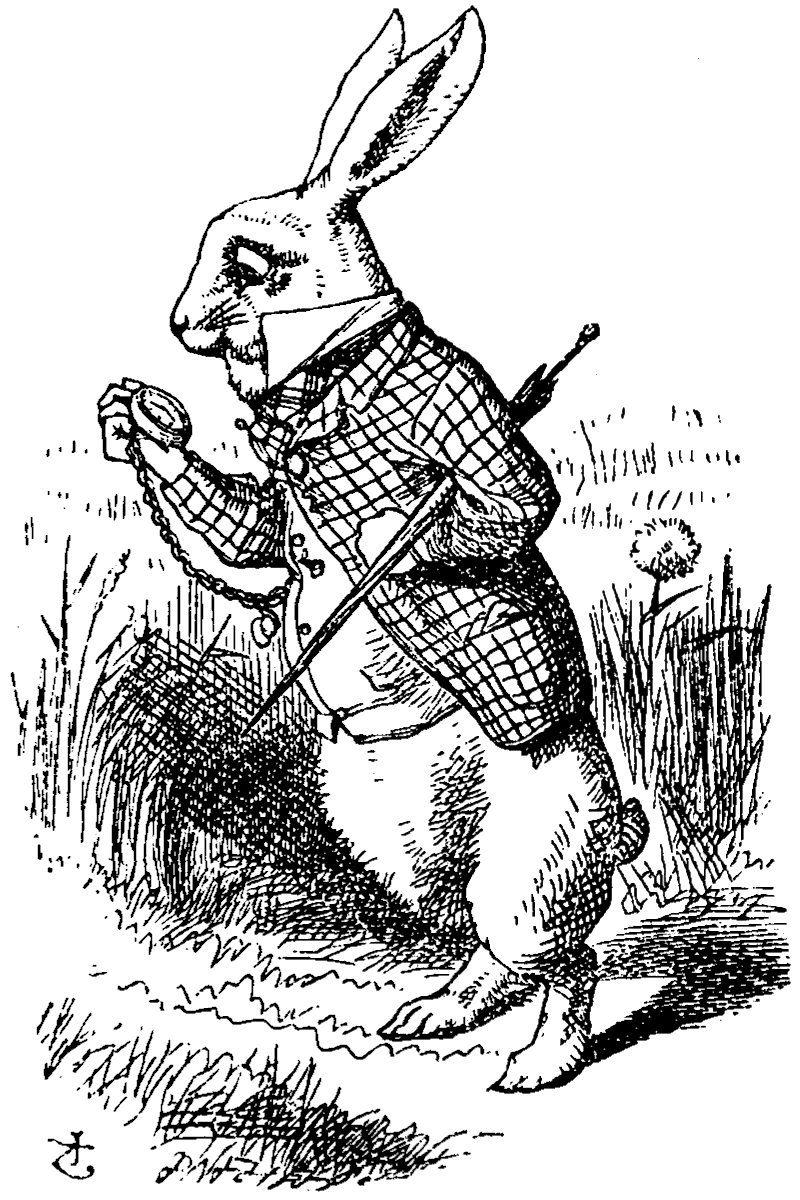
\includegraphics[scale=0.4]{assets/rabbit.png} \\ ``By a clock we understand anything characterized by a phenomenon passing periodically through identical phases so that \ldots all that happens in a given period is identical with all that happens in an arbitrary period.'' Albert Einstein}%16MHz
\section{Time}

\begin{frame}{Clocks}
	\begin{itemize}
		\item Quartz powered by a DC signal vibrates due to the piezoelectric effect at a reliable \textbf{reference frequency}. \\
			\begin{center} 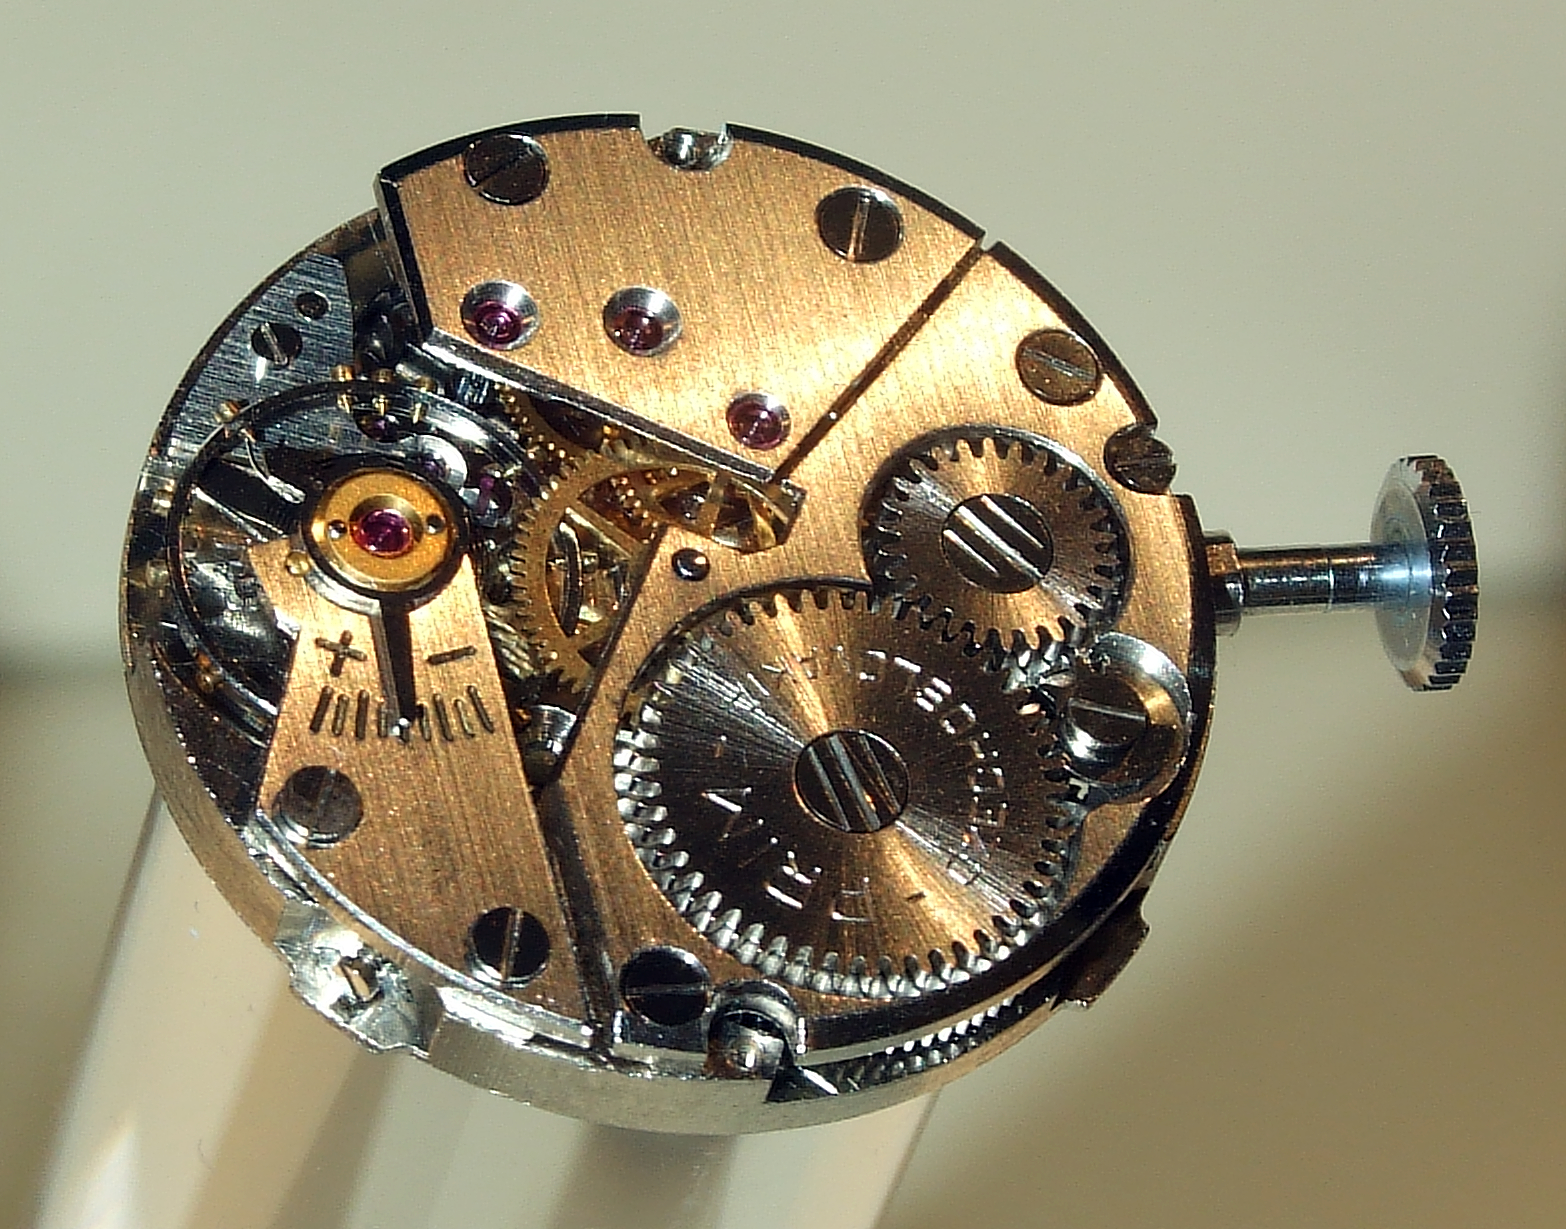
\includegraphics[scale=0.04]{assets/clockwork.jpg} 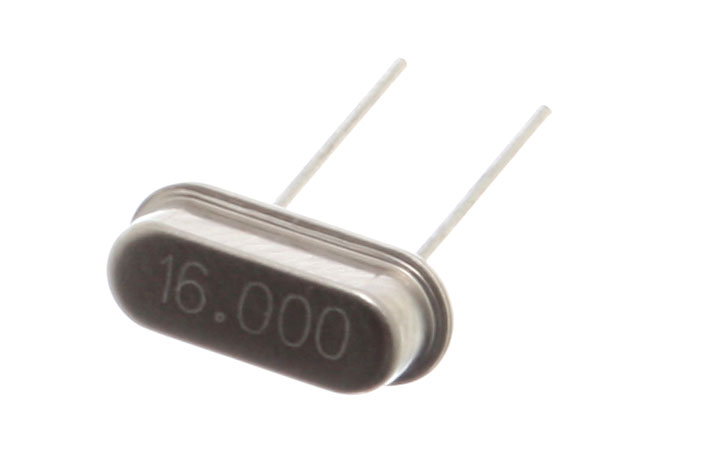
\includegraphics[scale=0.2]{assets/crystal.jpg} \end{center}
		\item A \textbf{voltage-controlled oscillator} has a frequency dependent on the input voltage.
		\item A \textbf{phase detector} can produce a signal whose strength depends on how fast or slow the VCO is running compared to the reference.
		\item If the VCO runs at a multiple of the reference frequency and is kept in a \textbf{phase-locked loop} with the reference, we can achieve oscillation at some multiple of the reference frequency. This can be chained a number of times.
	\end{itemize}
\end{frame}

\begin{frame}{Clock Drift}
	Heat, manufacturing differences, crystal aging, voltage fluctuations, etc., can cause two clocks $T_1(t)$ and $T_2(t)$ to experience \textbf{clock drift}, whereby $\theta_{1\to 2} = T_2(t)-T_1(t)$ changes over time.

	It is possible to observe negative apparent latency when naively comparing timestamps from poorly synced clocks.
	%graph for ES
	%Note that this is not trivial to distinguish from slow changes in service quality over time. But generally those are a bit more discrete
\end{frame}

\begin{frame}{Synchronisation}
	For synchronisation within a network we will typically have a time server with a \textbf{master clock}. This could be set just once or synced with some external source like GPS.

	\begin{center}
		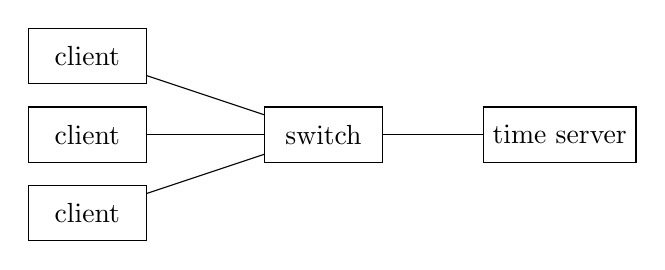
\begin{tikzpicture}[
		    node distance=2cm,
		    every node/.style={draw, rectangle, minimum width=1.5cm, minimum height=0.7cm}
		]
		    \node (switch) at (0,0) {switch};
		    \node (master) at (3,0) {time server};

		    \foreach \y in {1,0,-1} {
			\node (client\y) at (-3,\y) {client};
			\draw (client\y) -- (switch);
		    }

		    \draw (switch) -- (master);
		\end{tikzpicture}
	\end{center}

	Each piece of hardware can be equipped with its own clock $T_{*}(t)$.

	By sending messages across the network, recording timestamps at each of the clocks, and adjusting for latency, we can estimate the clock drift.

	This allows us to adjust the client clock speed (\textbf{slewing}) such that $\theta_{c\to m}$ approaches zero.
\end{frame}

\begin{frame}{Network Time Protocol}
	Using the \textbf{network time protocol} involves the client making requests to the time server that are labeled with four receive/transmit timestamps $T_c(t_1), T_m(t_2), T_m(t_3), T_c(t_4)$.

	Suppose we have symmetric latency $T_m(t_2)-T_m(t_1) = T_m(t_4)-T_m(t_3)$.
	It follows that $T_m(t_2)-(T_c(t_1)+\theta_{c\to m}) = (T_c(t_4)+\theta_{c\to m})-T_m(t_3)$. Then
	\begin{align*}
		\theta_{c\to m} &= \frac{1}{2}\left(\underbrace{(T_c(t_4)-T_m(t_3))}_\text{Receive} - \underbrace{(T_m(t_2)-T_c(t_1))}_\text{Transmit}\right) \\
		&= \frac{1}{2}\left(\underbrace{(T_c(t_4)-T_c(t_1))}_\text{Round-trip time} - \underbrace{(T_m(t_3)-T_m(t_2)}_\text{Wire-to-wire}\right) \\
	\end{align*}

	In the case where wire-to-wire latency is zero, this is also known as Einstein synchronisation.
\end{frame}

\begin{frame}{Precision Time Protocol}
	Because the latency added by a switch is nondeterministic, we can achieve greater precision by controlling for its contribution.

	Suppose we have $T_c(t_1), T_s(t_2), T_s(t_3), T_m(t_4), T_m(t_5), T_s(t_6), T_s(t_7), T_c(t_8)$.

	Then we have
	$$\theta_{c\to s} = \frac{1}{2}\left((T_c(t_8)-T_s(t_7)) - (T_s(t_2)-T_c(t_1))\right),$$
	$$\theta_{s\to m} = \frac{1}{2}\left((T_s(t_6)-T_m(t_5)) - (T_m(t_4)-T_s(t_3))\right),$$
	$$\theta_{c\to m} = \theta_{c\to s} + \theta_{s\to m}.$$

	We can either record a cumulative adjustment in the timing packets (transparent switch), or sync the switch to the master clock and then the client to the switch (boundary clock).
\end{frame}

\sectionquote{``Speed is the essence of war.'' Sun Tzu \\ ``Remote fountains are of little help to nearby fires.'' Han Fei}
\section{Distance}

\subsection{WAN}
\begin{frame}[fragile]{Internetworking}
Things that are further away usually take longer to get a reply from:
	\begin{lstlisting}[ basicstyle=\ttfamily\bfseries\scriptsize ]
> ping -c 3 192.168.0.109
PING 192.168.0.109 (192.168.0.109): 56 data bytes
64 bytes from 192.168.0.109: icmp_seq=0 ttl=64 time=2.593 ms
64 bytes from 192.168.0.109: icmp_seq=1 ttl=64 time=12.022 ms
64 bytes from 192.168.0.109: icmp_seq=2 ttl=64 time=53.092 ms

--- 192.168.0.109 ping statistics ---
3 packets transmitted, 3 packets received, 0.0% packet loss
round-trip min/avg/max/stddev = 2.593/22.569/53.092/21.924 ms

	\end{lstlisting}
	\noindent\rule{\linewidth}{0.4pt}
	\begin{lstlisting}[ basicstyle=\ttfamily\bfseries\scriptsize ]
> ping -c 3 46.17.63.250
PING 46.17.63.250 (46.17.63.250): 56 data bytes
64 bytes from 46.17.63.250: icmp_seq=0 ttl=30 time=403.366 ms
64 bytes from 46.17.63.250: icmp_seq=1 ttl=30 time=338.468 ms
64 bytes from 46.17.63.250: icmp_seq=2 ttl=30 time=336.076 ms

--- 46.17.63.250 ping statistics ---
3 packets transmitted, 3 packets received, 0.0% packet loss
round-trip min/avg/max/stddev = 336.076/359.303/403.366/31.172 ms
	\end{lstlisting}
%alt data
%this is in london

%also, the more work you do, the longer it will usually take
\end{frame}

\begin{frame}{Private Wide Area Network Links}
	1850: Paul Reuter establishes a carrier pigeon service between financial hubs in Germany and Belgium

	2010: Spread Networks lays an optic fiber network between Chicago and New Jersey

	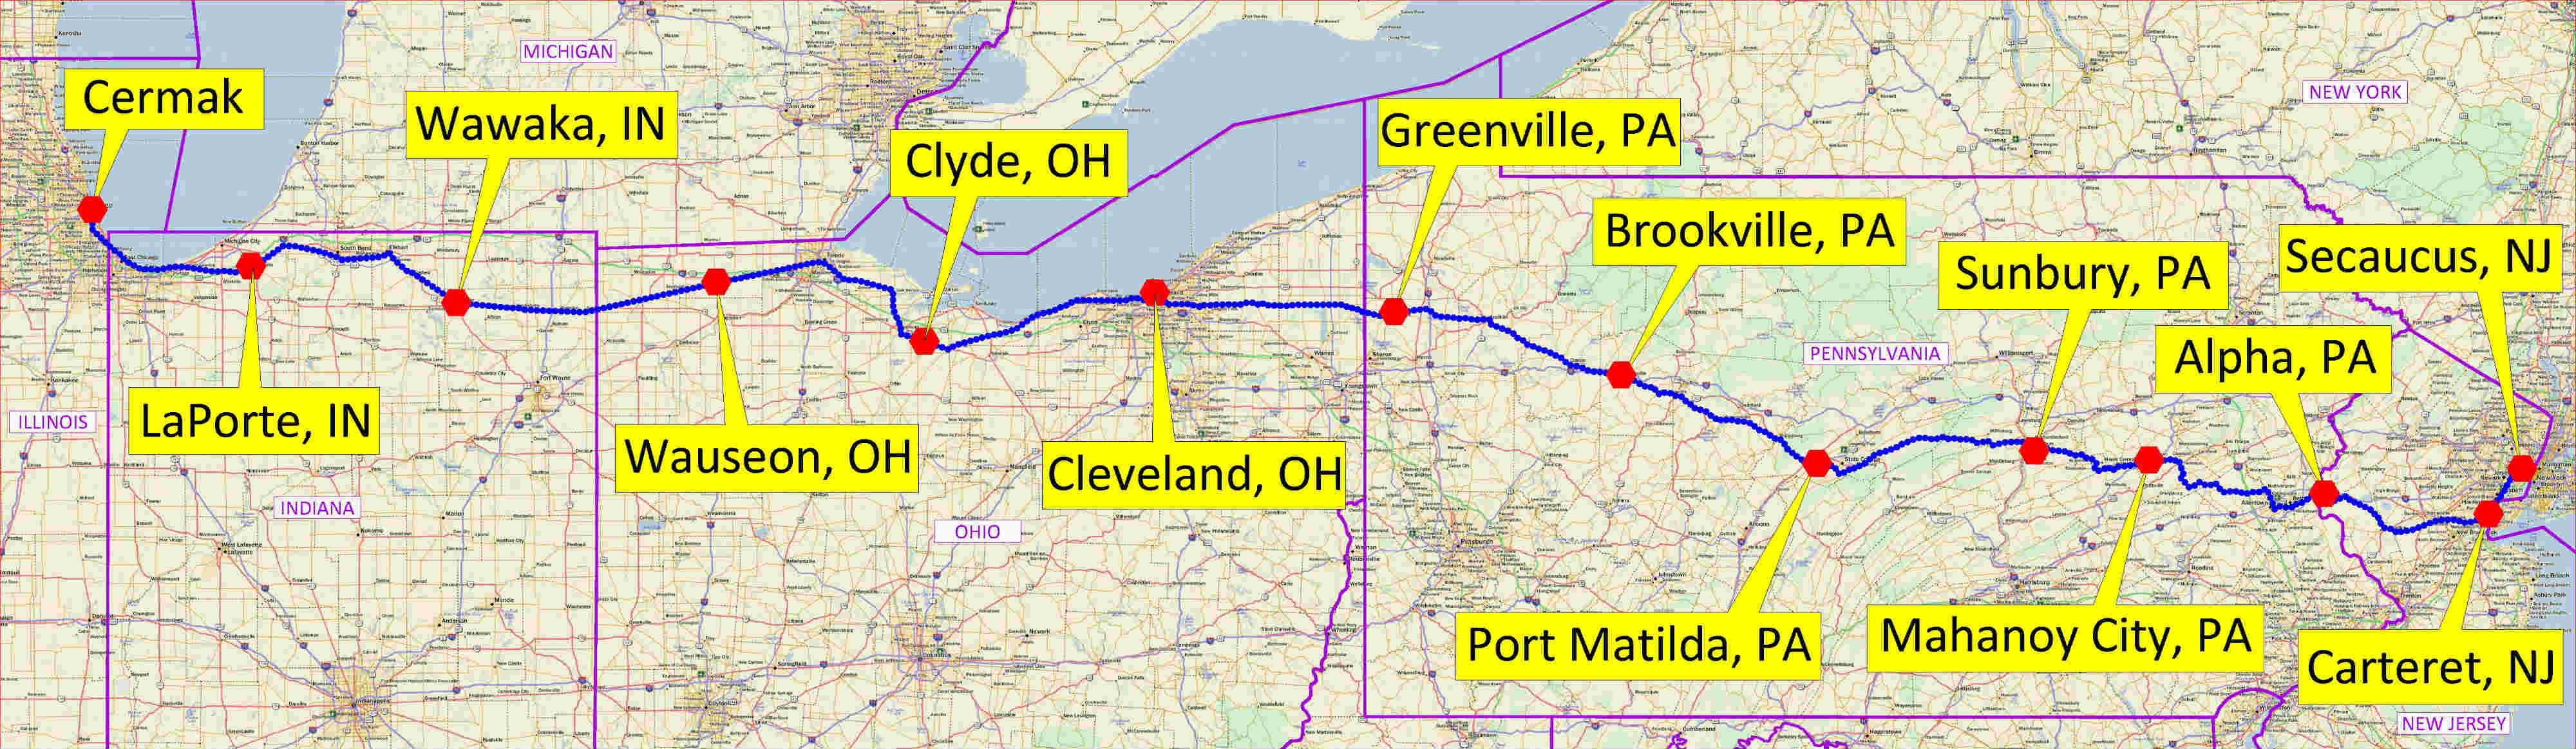
\includegraphics[scale=0.08]{assets/map.jpg}

	2012: McKay Brothers installs an overground microwave tower relay

	2017: Go West consortium consolidates fiber optic, microwave, and undersea cables between Chicago and Tokyo

	Supposedly, shortwave radio can be bounced off the ionosphere to traverse oceans faster than the speed of light in glass.
	% https://spectrum.ieee.org/wall-street-tries-shortwave-radio-to-make-highfrequency-trades-across-the-atlantic

	More recently, companies like SpaceX offer the ability to transmit at near-$c$ using inter-satellite links.
\end{frame}

\begin{frame}{Physical Media}
	Latency is either along the cable or on one of the ends.

	The longer the distance, the more we care about effects that scale linearly with distance.

	For private WAN links, we care mostly about the \textbf{propagation delay} of the medium, and the overhead required to remedy \textbf{attenuation}.
	%Rainy days might have less adverse selection in presence of microwave towers
	%Pictures of copper, fiber, and repeaters
	%fiber: single mode, multi-mode

	%throughput, PAM

	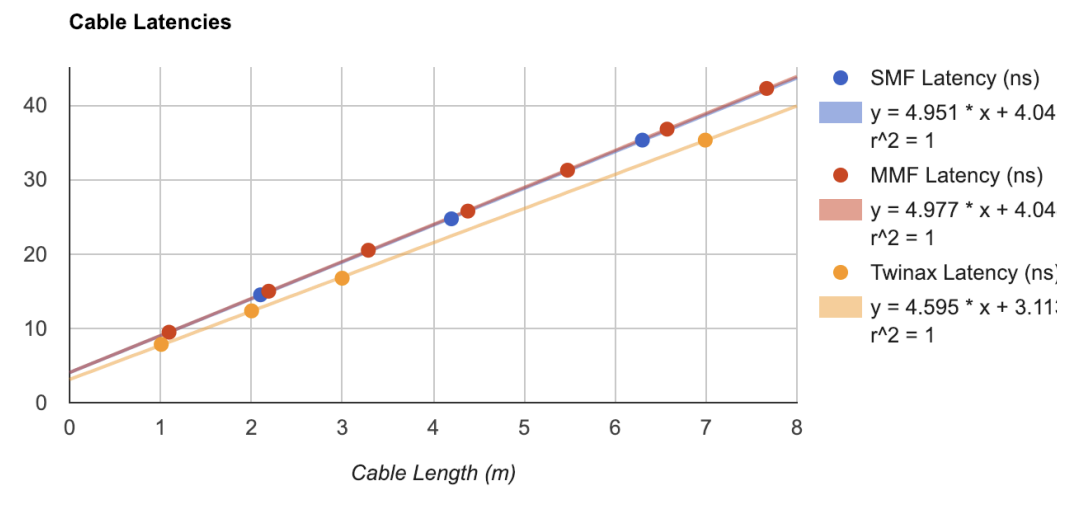
\includegraphics[scale=0.5]{assets/arista.png}
\end{frame}

\subsection{Colocation}
\begin{frame}{Direct Market Access}
	\begin{block}{}
		\scriptsize
		Remote connection $<$ Proximity hosting $<$ Primary colocation
	\end{block}
	%Also crypto eg AWS EC2
	%Equalisation is often a strong consideration especially when latency is very deterministic
	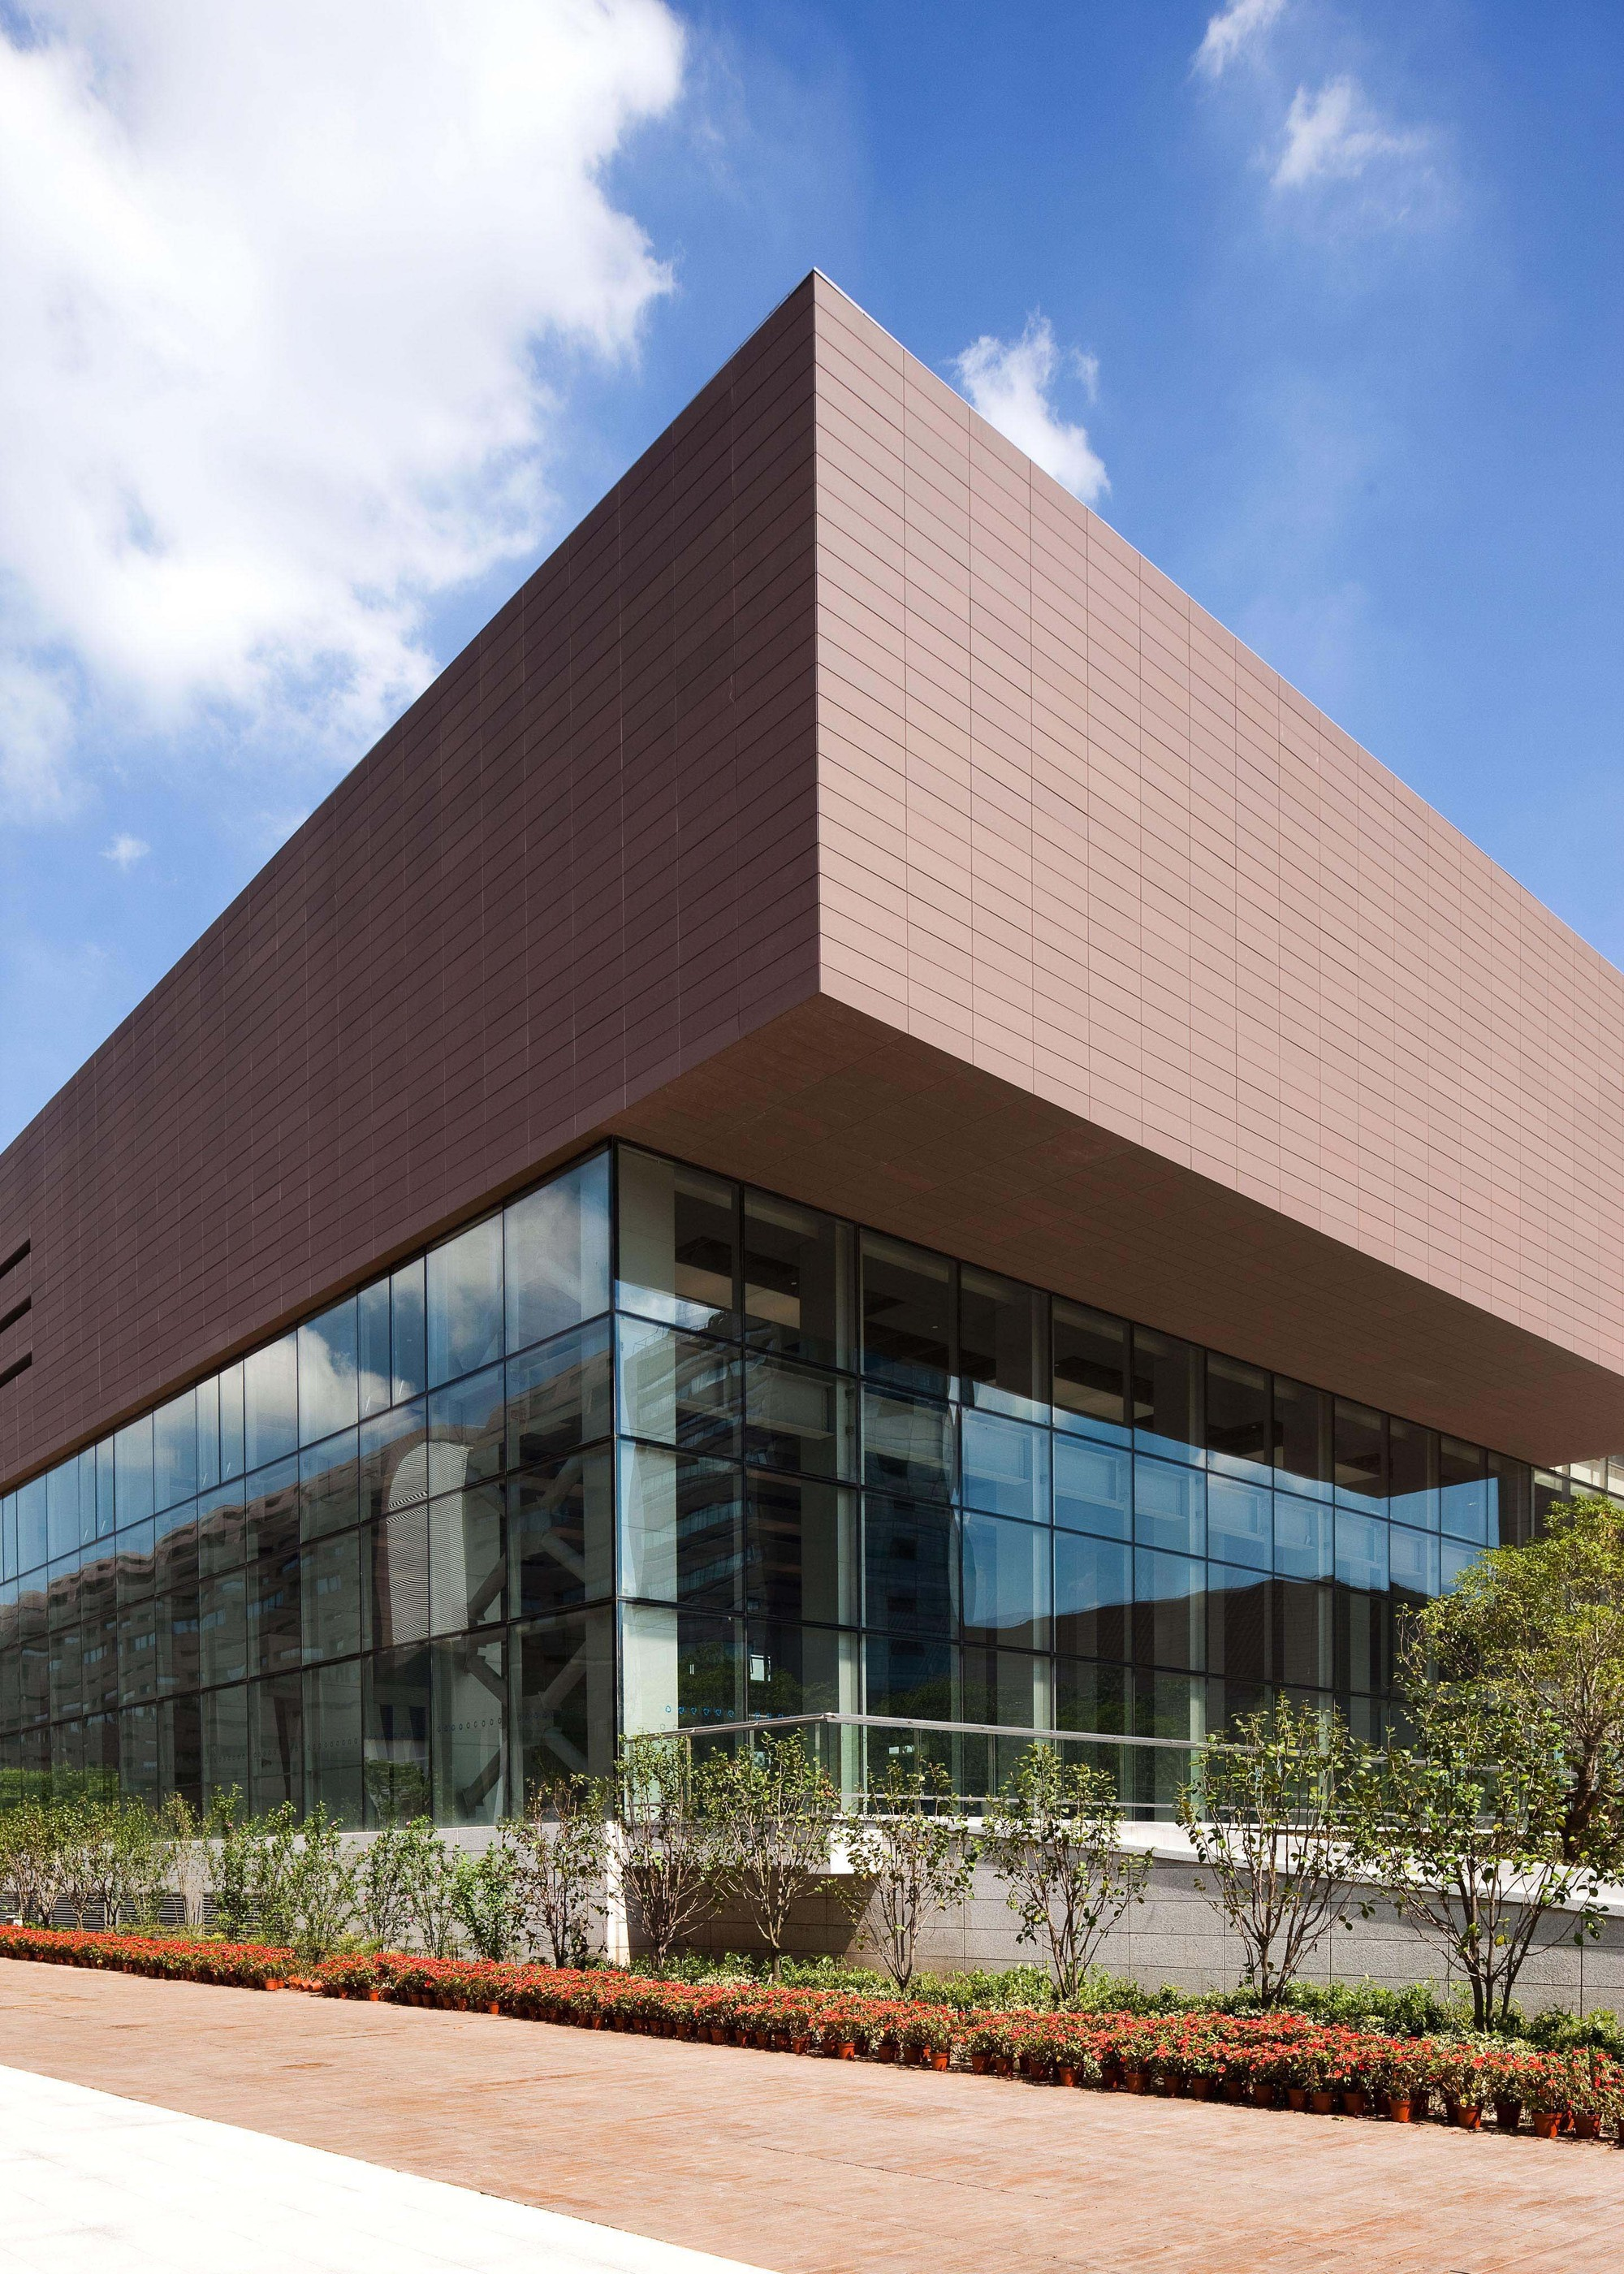
\includegraphics[scale=0.035]{assets/shfe.jpg}
	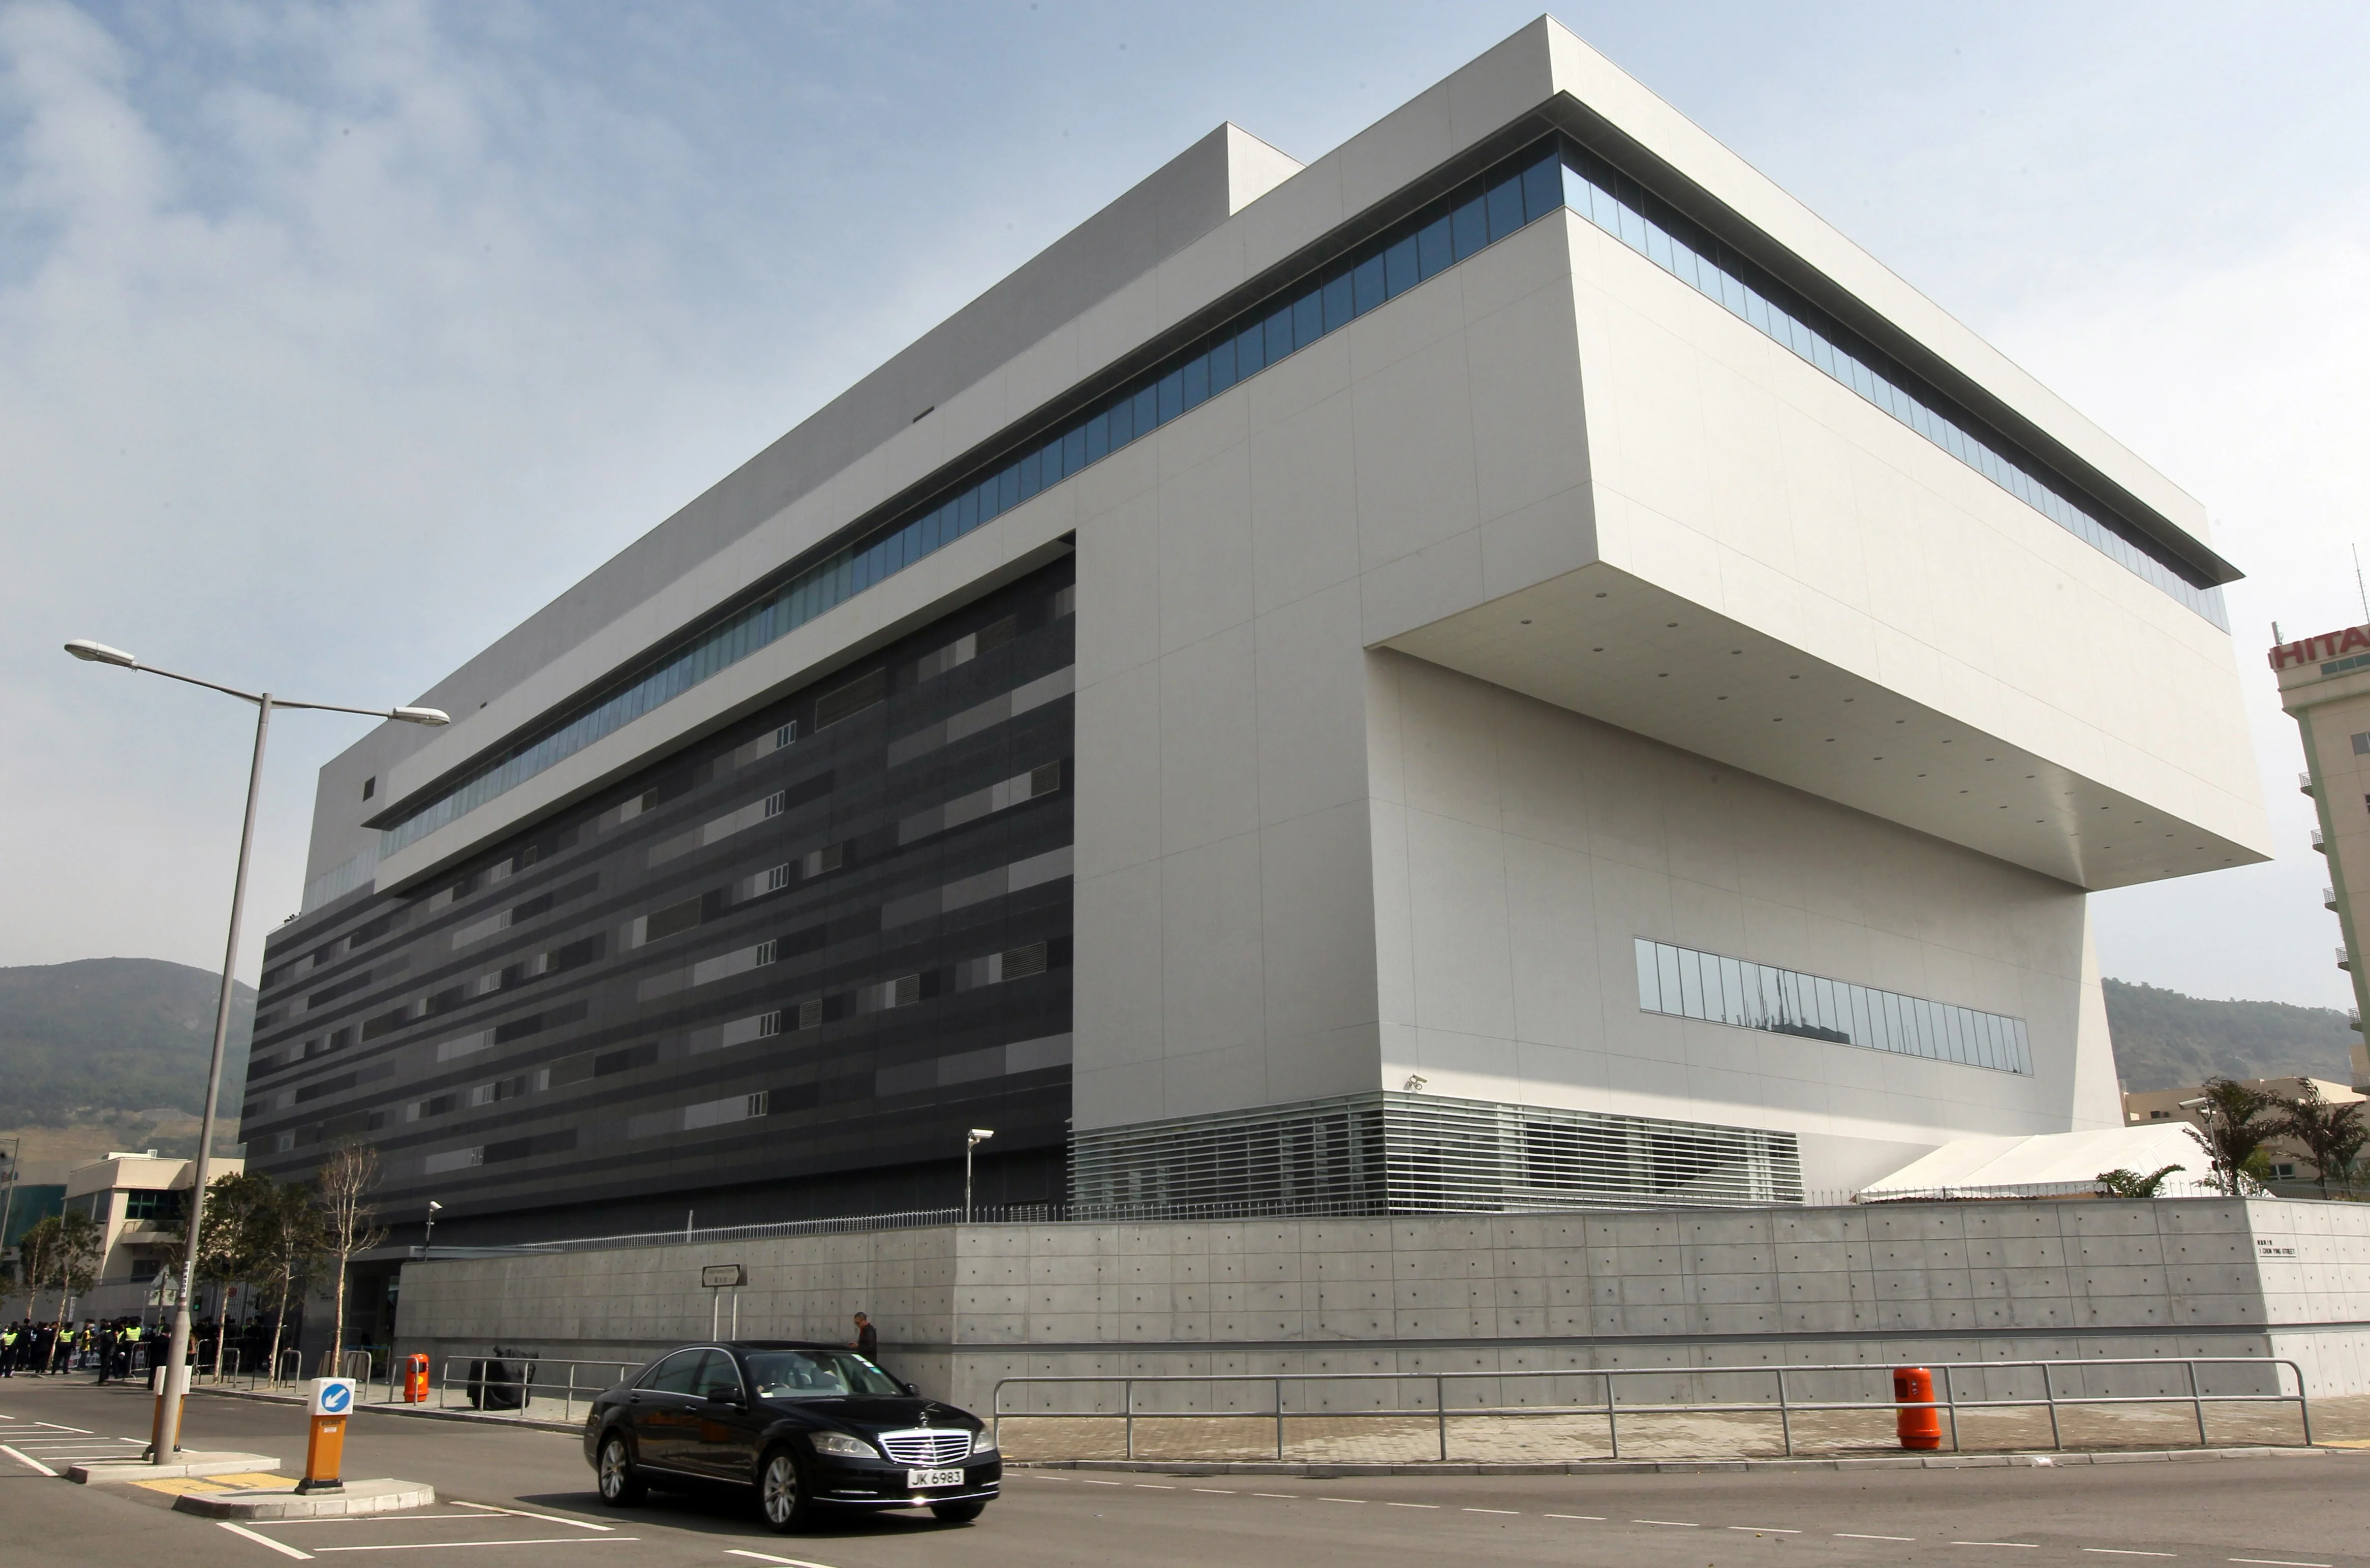
\includegraphics[scale=0.03]{assets/hkex.png}
	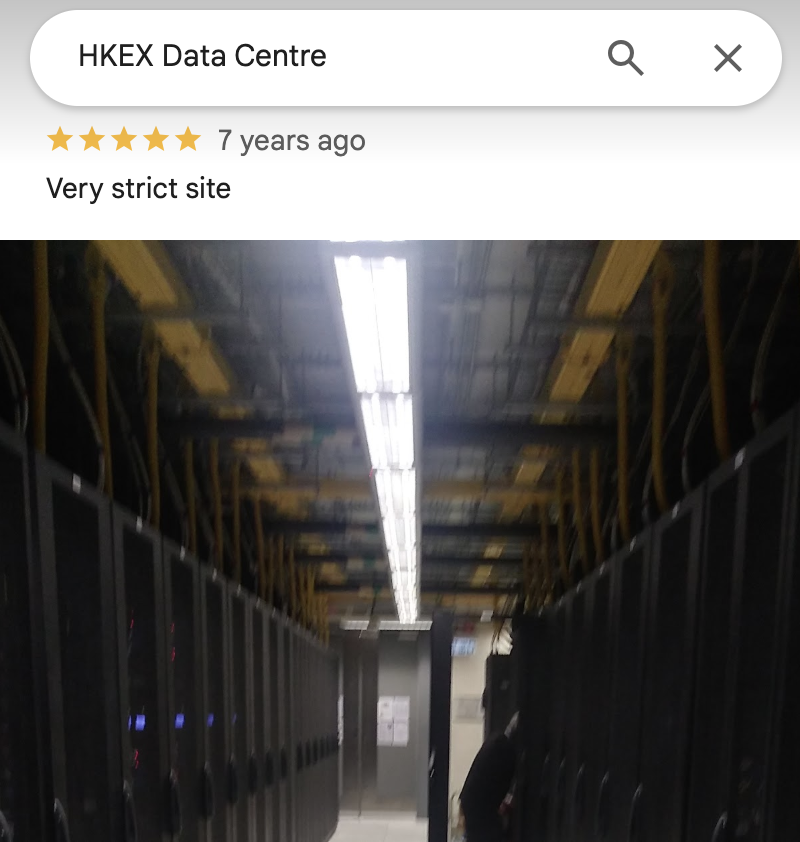
\includegraphics[scale=0.25]{assets/review.png}
	\pause
	\begin{block}{Jan 19 (Reuters)}
		\small
		China's securities regulator has asked brokers to remove client-dedicated servers from data centers in local exchanges, a move that will deprive rapid-trading "flash boys" of an edge against other investors, people with knowledge of the matter said.
		High-frequency traders in China have long used servers situated at data centers run by futures and stock exchanges and owned by brokers to execute trades as the physical adjacency shaves off milliseconds or even microseconds.
	\end{block}
	% https://www.reuters.com/world/china/china-curbs-flash-boys-access-exchange-data-sources-say-2026-01-19/
\end{frame}

\sectionquote{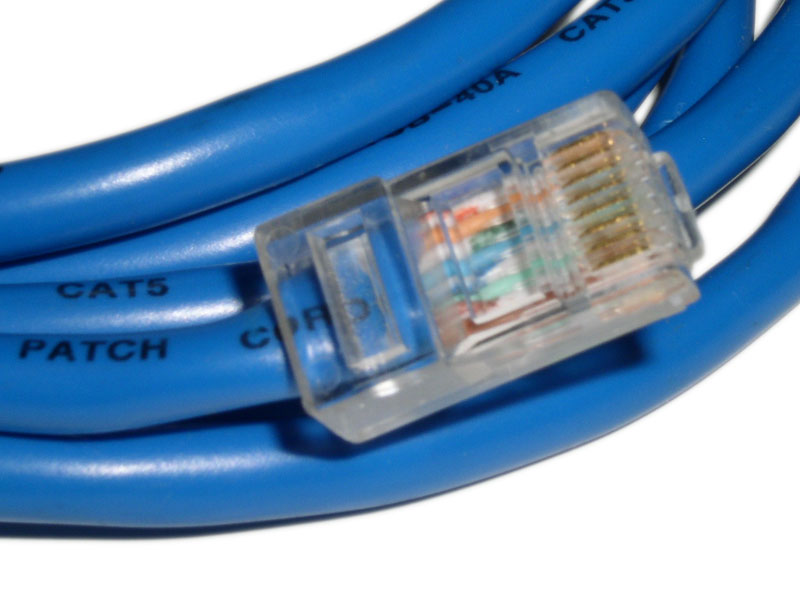
\includegraphics[scale=0.15]{assets/cat5.jpg} \\ ``This new form of communication could have some utility.'' Guglielmo Marconi \\ 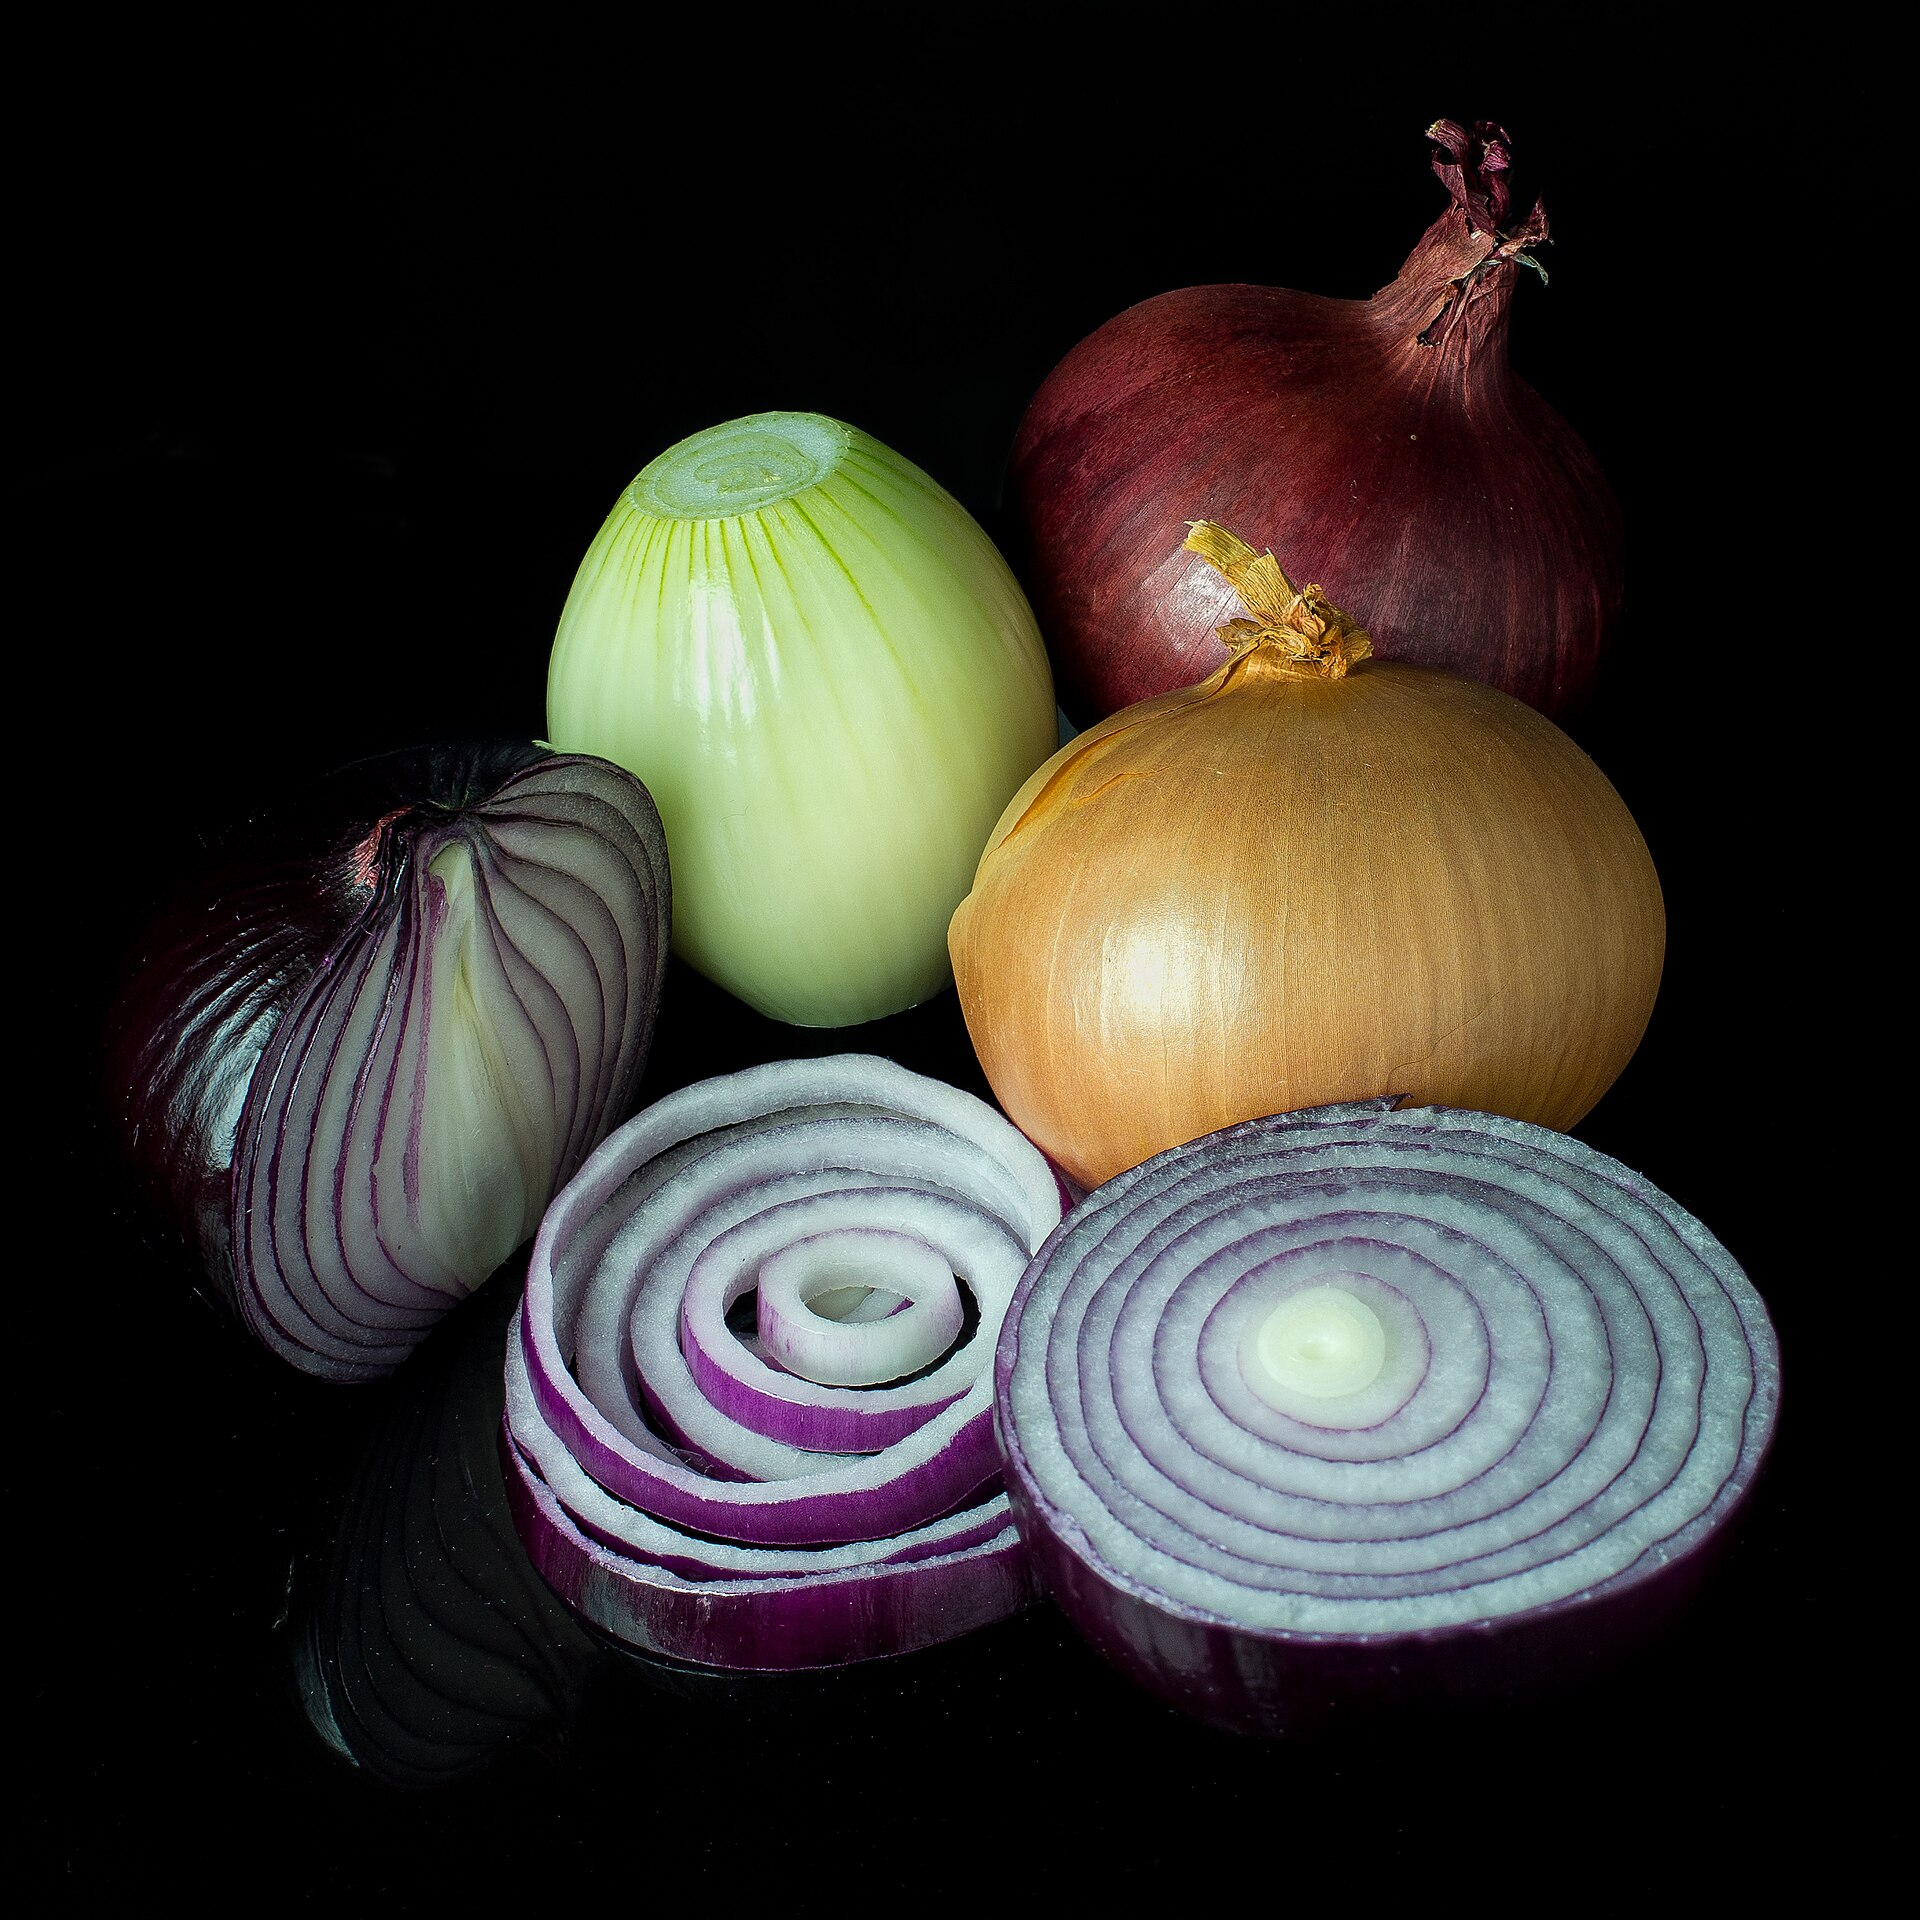
\includegraphics[scale=0.04]{assets/onion.jpg}}
\section{Networking}
\begin{frame}{Networking Stack}
	\centering
	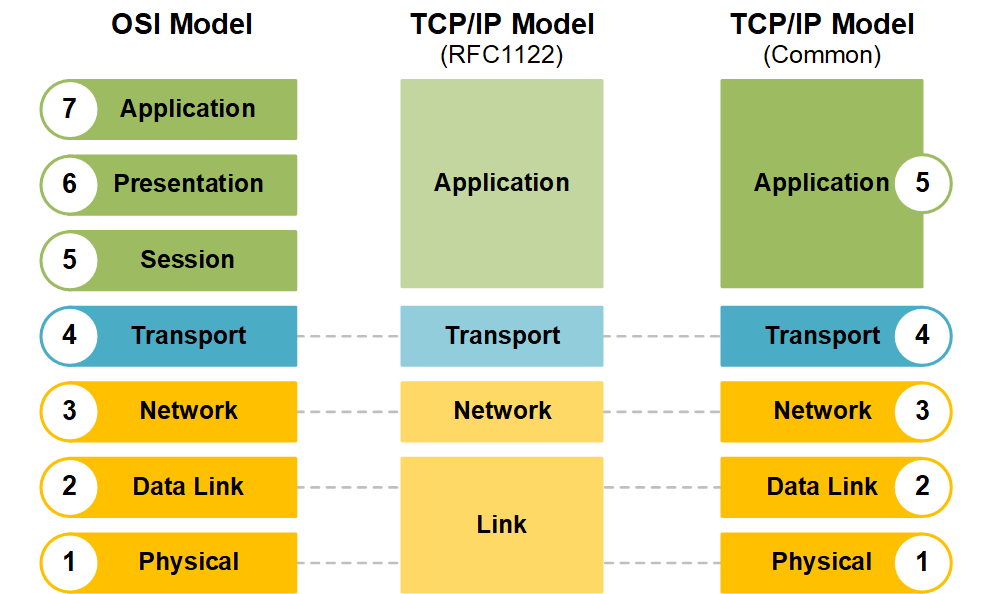
\includegraphics[scale=0.6]{assets/osi.png}
\end{frame}

\begin{frame}{Hardware}
	\begin{itemize}
		\item 1969: NPL network becomes operational, governed by a central `routing' computer rather than an L1 crosspoint
		\item 1977: Patent granted for Ethernet, introducing CSMA/CD
		\item 1986: HP announces StarLAN, one of the first Ethernet hubs.
		\item 1986: DEC introduces the LANBridge 100 with a software-level MAC table and selective casting.
		\item 1989: Kalpana introduces EtherSwitch with a hardware-level MAC table, allowing half-duplex cut-through switching
		\item 1995: Cisco releases the Catalyst 5000 switch, supporting multicast switching
		\item 1999: Cisco releases the Catalyst 6000 switch, supporting Pulse Amplitude Modulation
	\end{itemize}
	%Progress in many ways directed by commercial requirements different to those of HFT, so some of the older stuff still gets used
	%Why ``dark fiber'' matters. collisions, errors, duplex mismatch
	%Need a picture of generic network topology
\end{frame}

\begin{frame}{L2: Ethernet}
	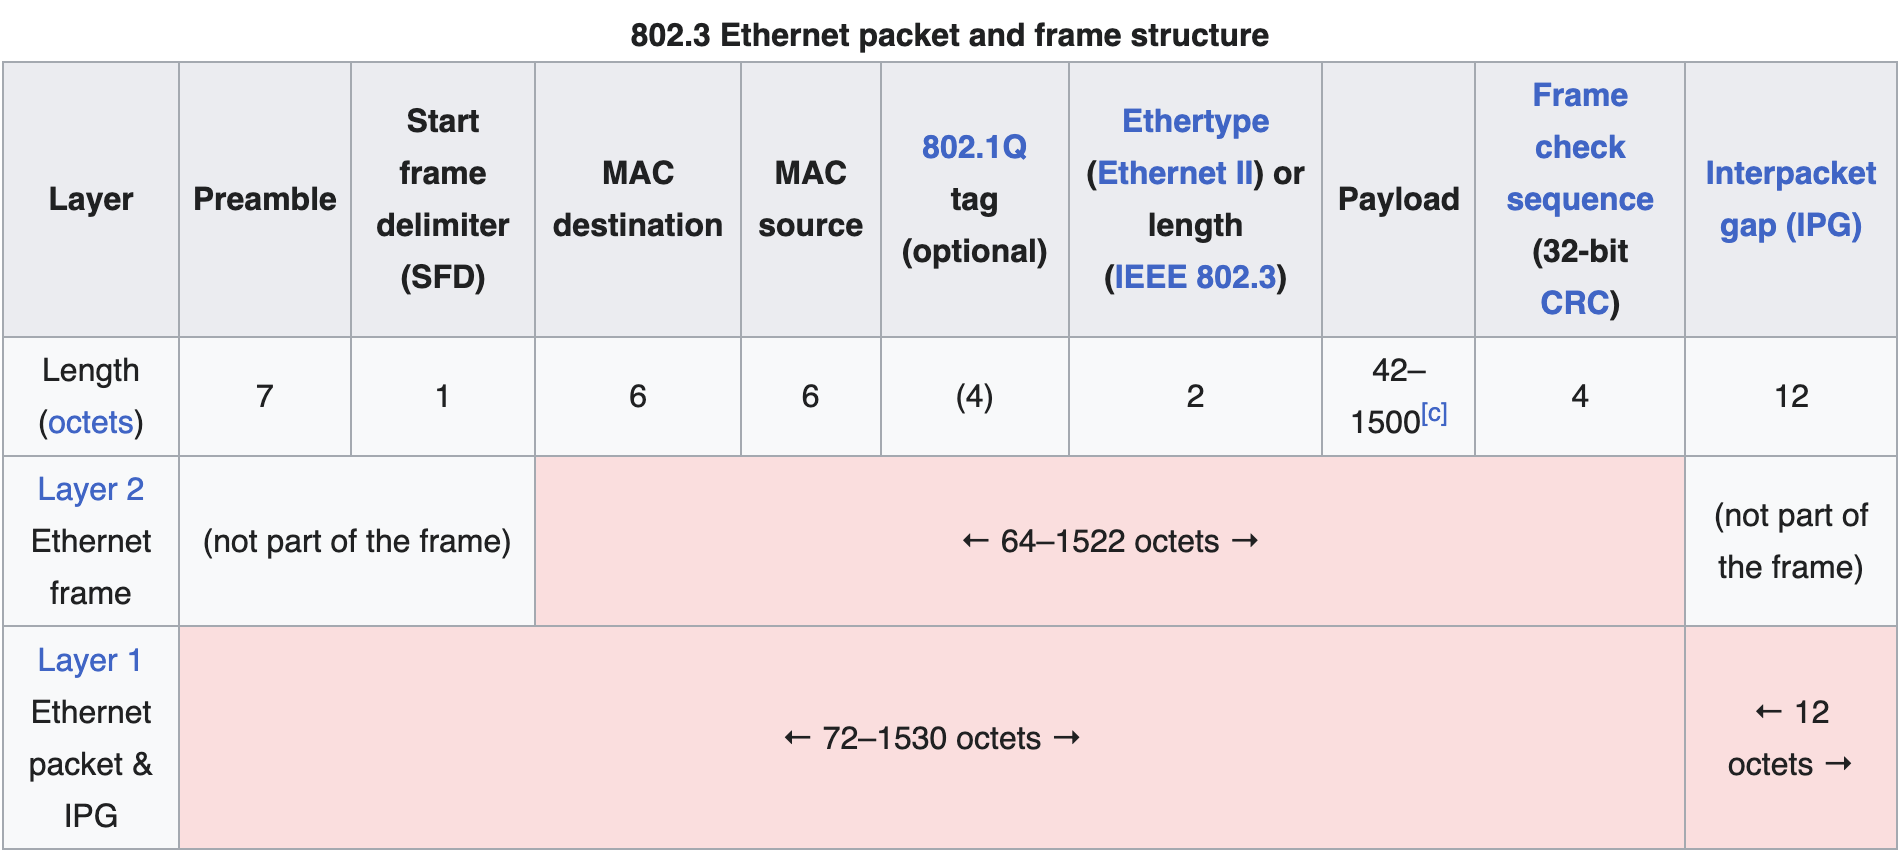
\includegraphics[scale=0.37]{assets/ethernet.png}
	%since we get size upfront maybe we can exploit this
	%jumbo frames - nonstandard
	%(uni/multi/broad)cast
	%use of mac address to identify maker of device
\end{frame}

\begin{frame}{L3: IP(v4)}
	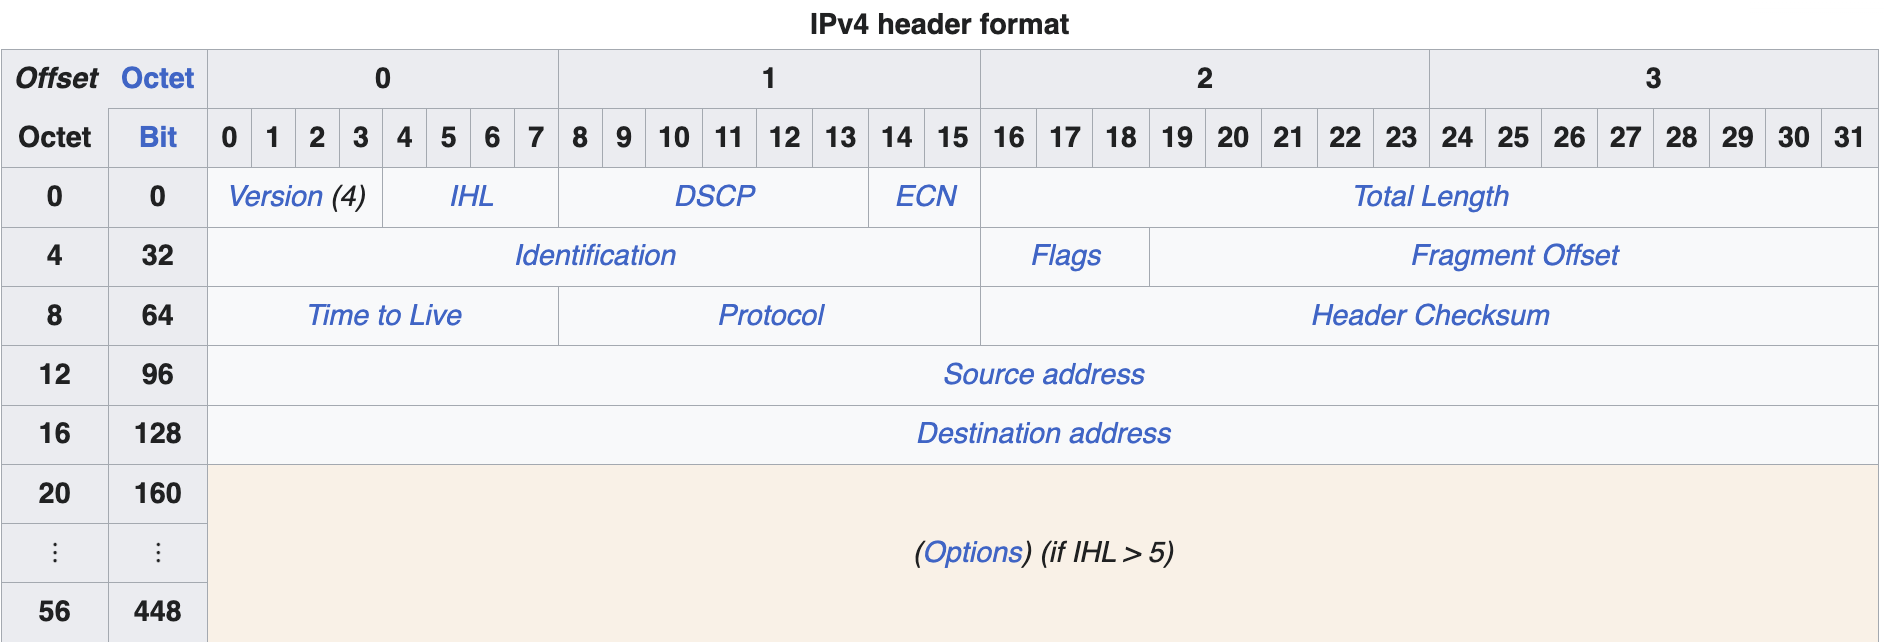
\includegraphics[scale=0.37]{assets/ipv4.png}
\end{frame}

\begin{frame}{L4: UDP}
	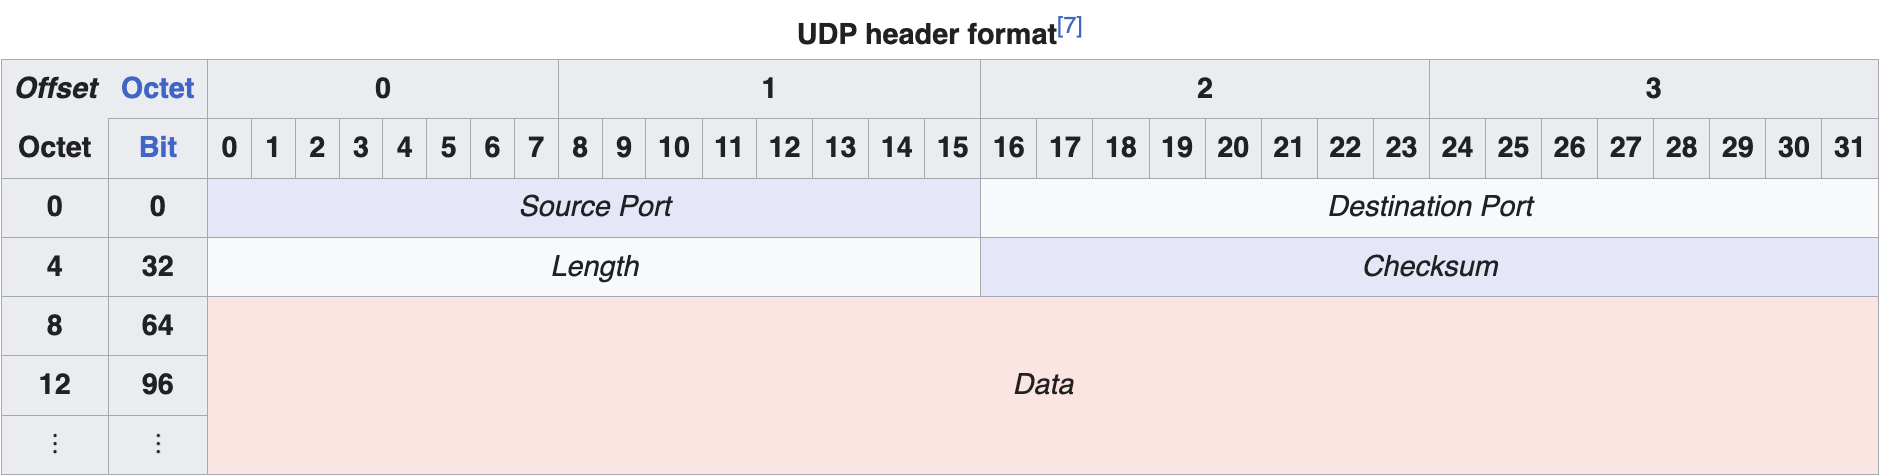
\includegraphics[scale=0.37]{assets/udp.png}
	%checksum depends on payload so might tell us something about the contents
	%PCAP Example
\end{frame}

\begin{frame}{L4: TCP}
	\begin{center}
		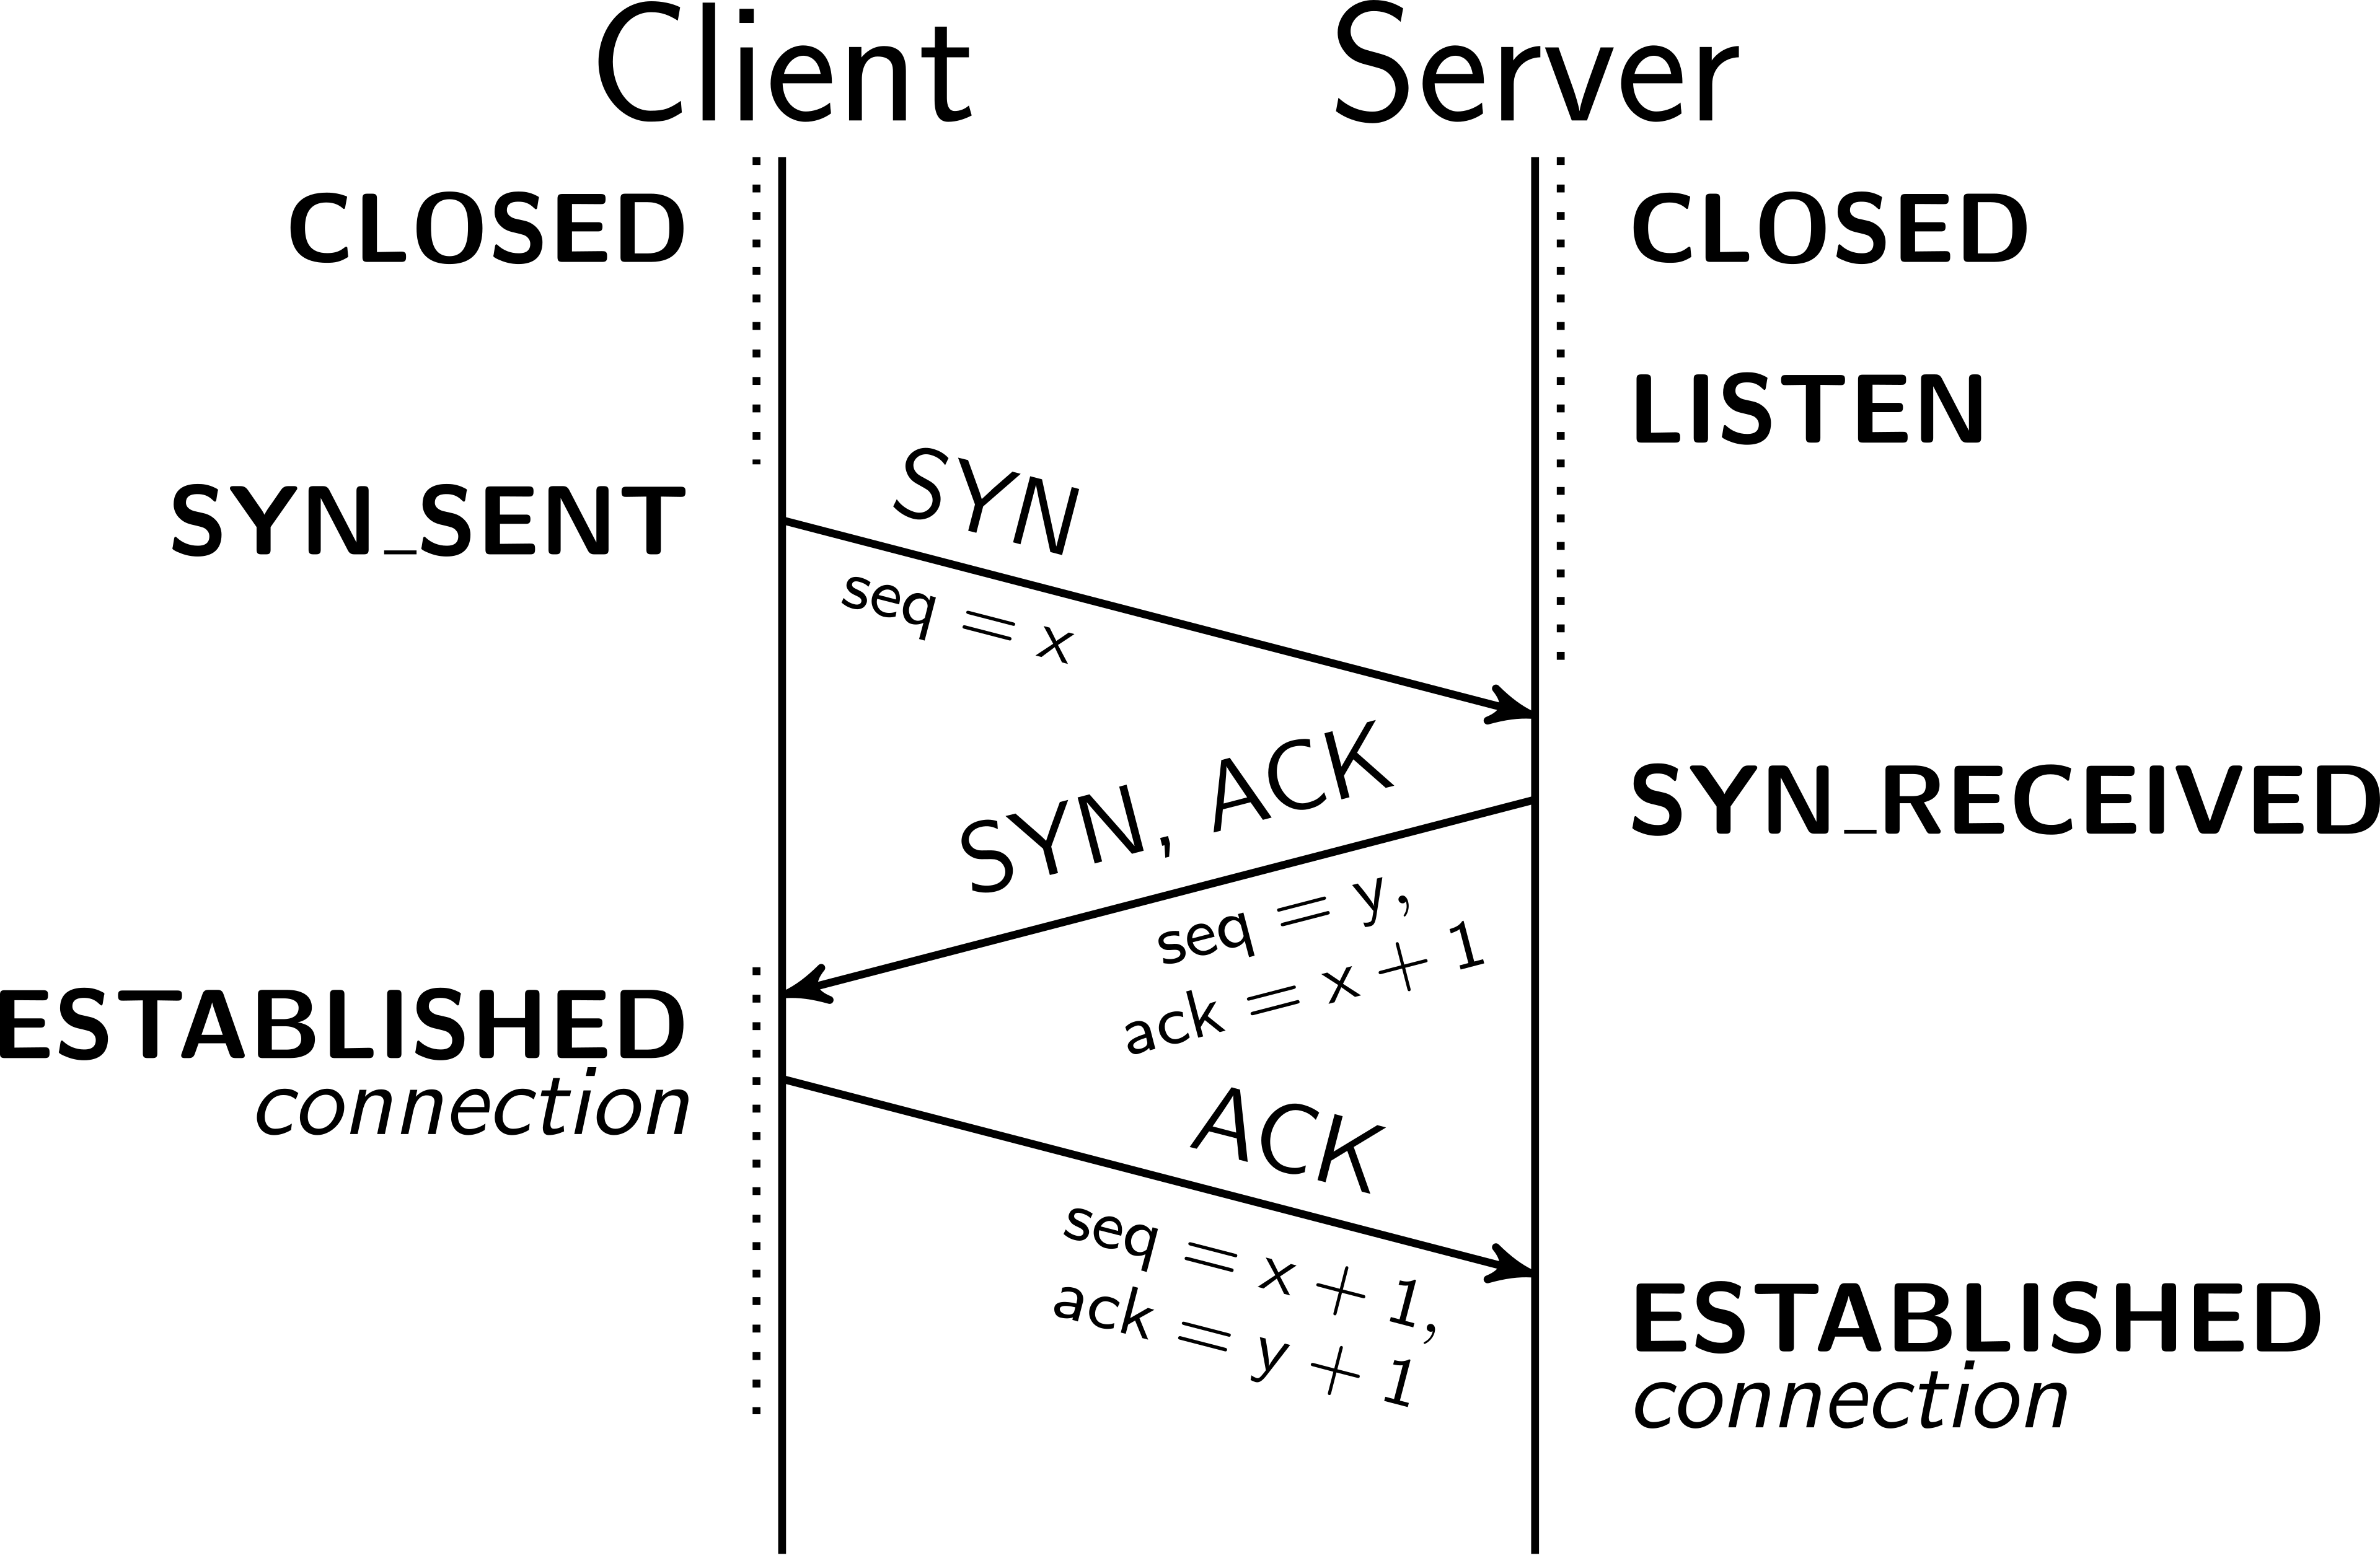
\includegraphics[scale=0.08]{assets/handshake.png}
	\end{center}
	%seq nums
\end{frame}

\begin{frame}{TCP Segment}
	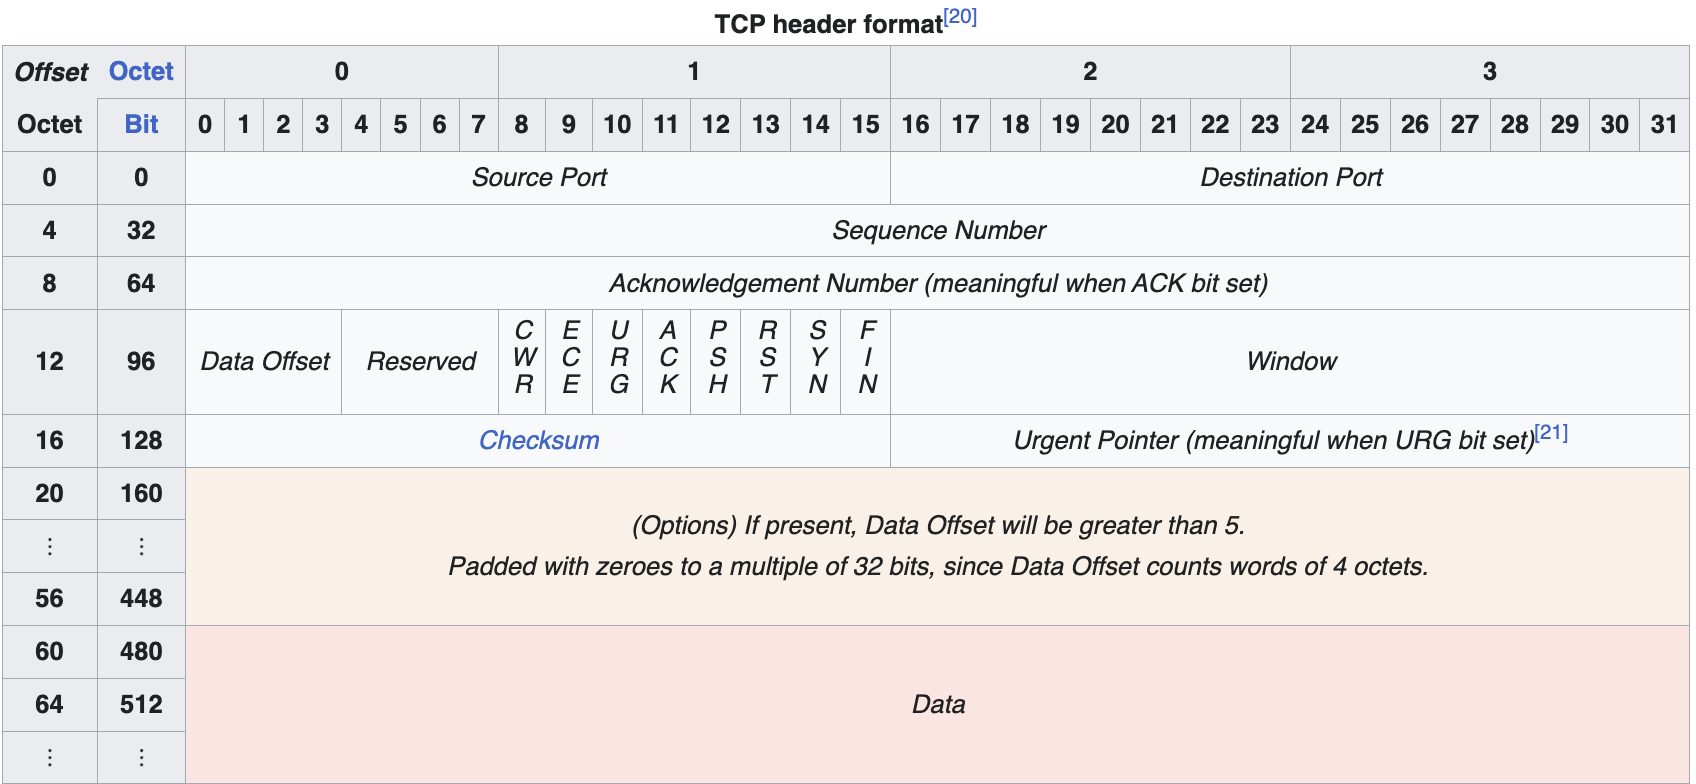
\includegraphics[scale=0.4]{assets/tcp.png}
\end{frame}

\begin{frame}{Exchange Protocols}
	%Execution
	%Market Data
	%ITCH, OUCH,OMNET,FIX
	% message structure, https://www.nasdaq.com/Options_Order_Feed
	% order types
\end{frame}

\begin{frame}{Network Timestamping}
	%Hardware vs software timestamping
	Timestamping of messages may be done at multiple points in the system (e.g. \texttt{timestamp\_match} and \texttt{timestamp\_publication}).

	Timestamps from different clocks (e.g. from different machines) are not trivial to compare owing to clock drift and clock sync inaccuracies (e.g. caused by network asymmetry).

	Usually the timestamp is calculated according to the first bit of the Ethernet header (start-of-frame). The last bit timestamp can be inferred using the bandwidth of the transmission.
\end{frame}

\begin{frame}{Abstract Colocation Topology}
	\diagram{}
\end{frame}

\begin{frame}{Example Colocation Topology}
	\centering
	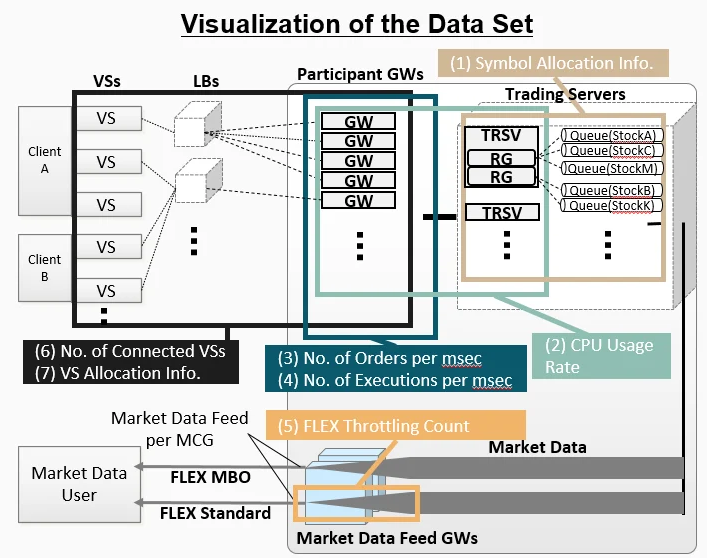
\includegraphics[scale=0.4]{assets/tse.png}
	%exchange documentation is a starting point but cannot always be fully trusted

	%https://www.reddit.com/r/chipdesign/comments/1arh2vr/what_is_a_phy/

	%https://en.wikipedia.org/wiki/Gateway_(telecommunications) - Gateways are servers. https://www.nasdaqtrader.com/Trader.aspx
\end{frame}

\part{Network Latency}
\begin{frame}{Part II: Network Latency}
	\tableofcontents[part=2]
\end{frame}

\sectiondiagram{execution}
\sectionquote{``We affirm that the world's magnificence has been enriched by a new beauty: \\the beauty of speed.'' Filippo Marinetti}
\section{Execution}

\begin{frame}{Externalities}
	\begin{block}{}
		``What if you want to be a bit more unpleasant? How about you work out \ldots \textbf{which is the best gateway to connect to?} \ldots You can start sending your orders through that.

		What about all these \textbf{other gateways}? What if you start stuffing orders through those other gateways that you don't care for matching? \ldots They're now \textbf{stuffed up with traffic} so other people can't compete.

		Then you go through the gateway that you have set up which you know is fast, and you're going to send your orders through nice and quick.'' Martin Thompson, \textit{Evolution of Financial Exchange Architecture} %https://www.infoq.com/presentations/financial-exchange-architecture/
	\end{block}
	%denial of service attack
	% idempotency
	% Compliance: "There is no such thing as compliance, only shades of commerciality." Because people often behave themselves and it is not so easy to tell when they don't, a lot of these regulations are never tested.

	\pause

	\textbf{Load balancers} help accomodate the large volume of data moving through the network, particularly during significant market events.

	Exchanges often impose limits on throughput (`\textbf{transactions per second}'). Limits might be per-session, per-user, etc.

	%https://news.ycombinator.com/item?id=30117637
\end{frame}

\begin{frame}{Compliance}
	\begin{block}{}
		In order to ensure every EP can trade in a fair and orderly market, activities including the following \ldots are therefore prohibited:
		\begin{enumerate}
			\item Deliberate fragmentation of Transmission Control Protocol (TCP) messages (‘packet splitting’);
			\item Deliberate retransmission of TCP or application layer messages;
			\item Deliberate transmission of corrupt network packets;
			\item Inappropriate/excessive use of non-trading messages such as heartbeat, connection management; and
			\item Hold up or interfere with normal queuing and processing of network or application messages.
		\end{enumerate}
	\end{block}
	% https://www.hkex.com.hk/-/media/HKEX-Market/Services/Circulars-and-Notices/Participant-and-Members-Circulars/SEHK/2025/CT08525E.pdf
\end{frame}

\begin{frame}{Fragmentation}
	\begin{block}{}
		``The virtual channels on the X.25 for ordering were only 64kbps – very slow. I figured we could hack those similarly \ldots and start filling out an order before we had one. This would save us milliseconds. You could turn the packet into something benign or invalid if you didn’t have an order.''

		Matt Hurd
	%Pre-sending, out-of-order sending, subsequent invalidation, etc.; concrete example
	\end{block}

	\begin{itemize}
		\item TCP/UDP protocol data units can be split across multiple Ethernet frames
		\item The recipient will hold these fragments for some time waiting for the rest of the PDU
		\item Ethernet preamble/FCS/IPG adds overhead
		\item Layer 4+ components like gateways will need to collect all the fragments before transmission continues
		\item Exchanges typically monitor packet corruption rates for signs of abuse
	\end{itemize}
	%switch types: cut-through, store-and-forward, buffering. How much latency is added by cut-through vs SAF, plus in case of many-to-one how much latency is added
	%ring-buffer design, multiple queues
	%favours small frames/packets, but then need more ethernet frame metadata including preamble. work through the maths. also: bandwidth != latency, relationship between latency and throughput, sharing bandwidth does not necessarily lead to latency
\end{frame}

\begin{frame}{Out-of-Order Delivery}
	Similarly, the use of sequence numbers in TCP makes it robust to out-of-order delivery of data:
	\begin{block}{}
		``We were already sending the first part of the message in an early packet.

		Why not \textbf{send the later part of the packet} with the next TCP sequence number plus one \textbf{and then send the middle part of the sequence out of order} with the symbol, price and quantity?

		That final part of the packet had quite a large user field so we would save an awesome amount of time and gain much more than we were with the speculative send we were already doing.''

		Matt Hurd
	\end{block}

	TCP guarantees delivery of a bytestream, and presentation-layer message boundaries need not align with packet boundaries.%In practice they often do
\end{frame}

\begin{frame}{Win-rate Modeling}
	%Probabilistic queueing models. https://en.wikipedia.org/wiki/Queueing_theory#External_links
	%store-and-forward congestion, backpressure, etc. ("The hurrier I go, the behinder I get." alice in wonderland)

	Suppose all participants have independent latency with mean $\mu_i$ and a common standard deviation $\sigma$ (also called \textbf{jitter}).

	If we model latency as a negative Gumbel distribution, the probability of being fastest is conveniently proportional to $\exp\left(\frac{\pi}{\sqrt{6}} \cdot \frac{-\mu_i}{\sigma}\right)$.
	%plot gumbel pdf

	If every participant sends $n_i$ independent copies of their message, the probability of being fastest is proportional to $n_i \cdot \exp\left(\frac{\pi}{\sqrt{6}} \cdot \frac{-\mu_i}{\sigma}\right)$.

	Of course, the latencies are usually not independent.
	%Gateway choice is a game
	\begin{center}
		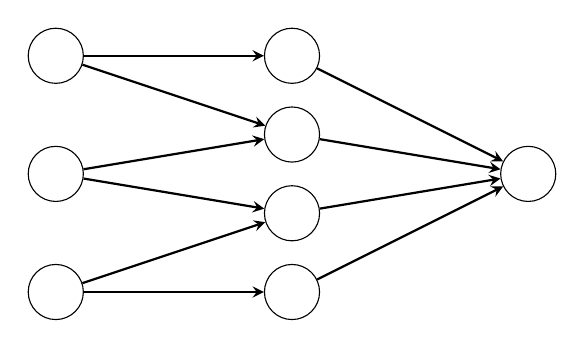
\begin{tikzpicture}[
		    >=stealth,
		    every node/.style={circle, draw, minimum size=7mm, inner sep=0pt},
		    arrow/.style={->, thick}
		]
			\node (a1) at (0, 1.5) {};
			\node (a2) at (0, 0) {};
			\node (a3) at (0,-1.5) {};

			\node (b1) at (3, 1.5) {};
			\node (b2) at (3, 0.5) {};
			\node (b3) at (3,-0.5) {};
			\node (b4) at (3,-1.5) {};

			\node (c1) at (6, 0) {};

			\draw[arrow] (a1) -- (b1);
			\draw[arrow] (a1) -- (b2);

			\draw[arrow] (a2) -- (b2);
			\draw[arrow] (a2) -- (b3);

			\draw[arrow] (a3) -- (b3);
			\draw[arrow] (a3) -- (b4);

			\draw[arrow] (b1) -- (c1);
			\draw[arrow] (b2) -- (c1);
			\draw[arrow] (b3) -- (c1);
			\draw[arrow] (b4) -- (c1);
		\end{tikzpicture}
	\end{center}
	%supermarket model
\end{frame}

\begin{frame}{Lottery Game}
	\begin{block}{}
		\begin{itemize}
			\item An online lottery website is offering a \$1m jackpot.
			\item Unfortunately, because they vibecoded the website, nobody is able to buy any tickets. Even worse, $n$ users have each been given one free ticket.
			\item Each number $i$ has some probability $p_i$ of winning, in which case the jackpot will be split equally amongst all players who chose $i$. If nobody wins, the jackpot will not pay out.
		\end{itemize}

		How should the players choose their numbers?
	\end{block}

\end{frame}

\begin{frame}{Lottery Game Solution}
	If a player chooses each number $i$ with probability $\pi_i$, and other players with probability $\pi_i'$, the player's expected payoff (in millions of dollars) is

	\begin{align*}
			& \pi_i \cdot p_i \cdot \left(\sum_{k=0}^{n-1}\frac{1}{1+k}\binom{n-1}{k} \pi_i'^k (1-\pi_i')^{n-1-k}\right) \\
		=	& \pi_i \cdot p_i \cdot \left(\sum_{k=0}^{n-1} \left(\int_0^1 x^k dx\right)\binom{n-1}{k} (\pi_i')^k(1-\pi_i')^{n-1-k} \right) \\
		=	& \pi_i \cdot p_i \cdot \int_0^1 \left(\sum_{k=0}^{n-1} \binom{n-1}{k} (\pi_i'\cdot x)^k (1-\pi_i')^{n-1-k} \right)dx \\
		=	& \pi_i \cdot p_i \cdot \int_0^1 (1 - \pi_i' + \pi_i'\cdot x)^{n-1} dx = \pi_i \cdot p_i \cdot \frac{1 - (1-\pi_i')^n}{n\pi_i'}.
	\end{align*}

	For a symmetric equilibrium, we require that $p_i \cdot \frac{1 - (1-\pi_i')^n}{n\pi_i'}$ is the same for all $i$. If $(1-\pi_i')^n$ is negligible this reduces to $\pi_i'\propto p_i$.
\end{frame}

\sectiondiagram{matching}
\sectionquote{``The most amazing achievement of the computer software industry is its continuing cancellation of the steady and staggering gains made by the computer hardware industry.'' Henry Peteroski}
\section{Matching Engine}

\begin{frame}{Matching Engine Responsibilities}
	\begin{itemize}
		\item Handle trading session initialisation and publication of reference data
		\item Capture messages from the network and assign an order in which they are to be processed
		\item Parse and validate messages, including risk checks
		\item Apply valid changes to \textbf{alter the order book state}
		\item \textbf{Produce trades} when appropriate conditions are met
		\item Log market events for clearing \& regulatory review
		\item Publish market events \& order status back to participants
		\item Handle heartbeats, disconnects, and recovery
	\end{itemize}
\end{frame}

\begin{frame}{Matching Engine Requirements}
	The main goal of matching engine design is \textbf{reliability}. For the exchange, latency is a secondary consideration.
	\begin{itemize}
		\item Throughput under worst-case load
		\begin{itemize}
			\item Load balancing
			\item Multi-threaded validation/parsing
			\item Sharding/partitioning %but consider risk checks, combo books. cross-product congestion
			\item Caching
		\end{itemize}
		\item Continuous availability
		\begin{itemize}
			\item Live backup server
			\item Heartbeat messages
		\end{itemize}
		\item State machine determinism
		\begin{itemize}
			\item Single-threaded transaction processing
		\end{itemize}
		\item Fairness
	\end{itemize}
	\begin{block}{}
		``The transition to TCP was a little messy \ldots Sometimes the feed imbalances would have severe delays, with data lagging behind tens of minutes. Once the imbalance cleared, the engines would automatically go back to trading.''

		Matt Hurd
	\end{block}
\end{frame}

\begin{frame}{Order Book Representation}
%CLOB. Priority. How to efficiently maintain.
%efficient matching engine https://arxiv.org/html/2606.01183v1
\end{frame}
%self-match prevention & cancellation disadvantage

%Dynamic gateway selection
%Gateway cache eviction -> warming

%Adverse selection: arises when edge reqs are different for instance

%EC2 instance that handles a matching engine, a BTC WAN link, and external order entry (dumber, slower participants)
%Two EC2 instances (taker-only, market-maker) that compete for taking. MM risk limits naturally cause tradeable prices to move in the direction of dumb flow (eg based on stale base prices) regardless of fair value.
%Subscriber with dashboard for order book + btc price, P&L (taker-only vs maker) etc. plus tuning knobs for the players and the matching engine

\sectiondiagram{market}
\sectionquote{``The race is not to the swift, nor the battle to the strong \ldots but time and chance happeneth to them all.'' Ecclesiastes \\ ``The race is not always to the swift, nor the battle to the strong – but that’s the way to bet.'' Anon.}
\section{Market Data}
\begin{frame}{Market Data Types}
	\begin{block}{Public Feed}
		\begin{itemize}
			\item Trades
			\item Depth
			\begin{itemize}
				\item L1: Best Bid/Offer (BBO)
				\item L2: Level sizes
				\item L3: Market-by-order%can use order ID to identify icebergs
				\item Incremental
				\item Snapshot
			\end{itemize}
		\end{itemize}
	\end{block}
	\begin{block}{Private Feed}
		\begin{itemize}
			\item Fills
			\item Acknowledgement of order creation/deletion
		\end{itemize}
	\end{block}

	Often we will get the same information in more than one way. 
%## Feed Arbitration
% https://ieeexplore.ieee.org/document/6718377
\end{frame}

\begin{frame}[fragile]{Trade Message Example (\href{https://api2.sgx.com/sites/default/files/2026-06/OMnet_MessRef_SGX_va42.pdf}{SGX OMnet})}
\begin{lstlisting}[ basicstyle=\ttfamily\bfseries\tiny ]
struct BD70 { // Trade Ticker VIB (Variable Information Broadcast)
	struct broadcast_hdr {
		struct broadcast_type {
			CHAR central_module_c; CHAR server_type_c;
			UINT16_T transaction_number_n // Transaction Type Number
		}
		UINT16_T items_n // Items
		UINT16_T size_n // Size
	}
	struct sub_item_hdr {
		UINT16_T named_struct_n // Named Struct, Number
		UINT16_T size_n // Size
	}
	struct basic_trade_ticker { // Named struct no: 34401
		struct series { // Named struct no: 50000
			UINT8_T country_c; UINT8_T market_c; UINT8_T instrument_group_c;
			UINT8_T modifier_c; UINT16_T commodity_n; UINT16_T expiration_date_n;
			INT32_T strike_price_i
		}
		struct timestamp_match { UINT32_T tv_sec; INT32_T tv_nsec }
		struct time_of_publication { UINT32_T tv_sec; INT32_T tv_nsec; }
		UINT64_T execution_event_nbr_u // Execution number %sequence number
		UINT32_T match_group_nbr_u // Match group number, group inside an execution %notably we dont know how many broadcasts are to come
		INT64_T deal_quantity_i // Quantity, Deal
		INT32_T deal_price_i // Price, Deal
		UINT16_T segment_number_n // Segment Number
		UINT8_T aggressive // Bid or Ask ; Of type: BID_OR_ASK_C
		CHAR filler_1_s // Filler
	}
}
\end{lstlisting}
\end{frame}

\begin{frame}[fragile]{Private Fill Message Example}
\begin{lstlisting}[ basicstyle=\ttfamily\bfseries\tiny ]
struct BO5 { // Firm Order Book VIB
	struct broadcast_hdr { ...  }
	struct sub_item_hdr { UINT16_T named_struct_n; UINT16_T size_n }
	struct trade_report_1_trans { // Named struct no: 34021
		struct transaction_type {
			CHAR central_module_c; CHAR server_type_c;
			UINT16_T transaction_number_n // Transaction Type Number
		}
		struct series { ...  }
		struct order_var {
			INT64_T mp_quantity_i; INT32_T premium_i; UINT32_T block_n;
			UINT16_T time_validity_n; UINT16_T exch_order_type_n;
			UINT16_T trigger_order_time_validity_n; char[16] ex_client_s;
			char[15] customer_info_s; UINT8_T open_close_req_c;
			UINT8_T bid_or_ask_c; UINT8_T ext_t_state_c;
			UINT8_T order_type_c; UINT8_T stop_condition_c; char[2] filler_2_s;
%Metadata, look for patterns. https://security.stackexchange.com/questions/216369/is-exposing-enumerated-ids-a-bad-idea-if-precautions-are-taken check databento sample PCAPs to see if obvious
		}
		struct party {char[2] country_id_s; char[5] ex_customer_s; CHAR filler_1_s}
		CHAR[32] exchange_info_s // Exchange, Information
		struct give_up_member {
			char[2] country_id_s; char[5] ex_customer_s; CHAR filler_1_s;
		}
		char[8] settlement_date_s // Date, Settlement
		char[8] time_of_agreement_date_s // Time of agreement, date part
		char[6] time_of_agreement_time_s // Time of agreement, time part
		UINT8_T deferred_publication_c // Deferred Publication
		CHAR filler_1_s // Filler
	}
}
\end{lstlisting}
\end{frame}
%If private feed is processed on a separate thread to market data, it can cause interpacket gap to depend on N
%Demo: Burstiness -> added latency, private feed (acks, traded, canaries)

%Market data: incremental, snapshot, etc. 
% https://medium.databento.com/analyzing-private-fills-and-canary-orders-with-databentos-high-precision-market-data-timestamps-8cb12f82a1a3

\begin{frame}{Publication Latency}
	\begin{itemize}{}
		\item During a burst of activity, the ME may need to do post-processing of data prior to sending.
		\item More complex transactions may take longer to be processed by the matching engine, or to traverse through the network.
		\item Larger messages may be \textbf{packetised} (L4) and packets may be \textbf{fragmented} (L2/L3)
		%Can correlate with things we don't see
	\end{itemize}
\end{frame}

\begin{frame}{Public Market Data}
	This is ideally \textbf{multicast} (or broadcast) to participants depending what kinds of feeds and products they choose to subscribe to.

	\begin{block}{}
		``At one later site \ldots we put in market data and it was the worst. \ldots We asked for this market data to be removed. A month or two later we paid for it to be reinstalled \ldots and now it was one of the best. \ldots I suspect some new kind of semi-permanent \textbf{round robin} positioning somewhere fixed things. There was little rhyme nor reason for many things.''

		Matt Hurd
	\end{block}

	%For fairness and latency reasons, public market data is ideally emitted only once by the matching engine NIC, then sent to a multicast switch that transmits to all relevant recipients simultaneously. Once received, packets can be further filtered or triaged by participants.

	%Nagle's algorithm, TCP_NODELAY https://brooker.co.za/blog/2024/05/09/nagle.html

\end{frame}

\begin{frame}{Private Feed}
	\begin{itemize}
		\item This is typically \textbf{unicast}, and the matching engine may need to decide on some reasonable order in which to send updates to participants.
		\item Depending on how this is achieved, there might be ways to gain priority in the distribution of private feed messages.
		\item Because only certain events emit private feed information, different styles of trading will be more or less likely to result in a private update about latency-sensitive events.
	\end{itemize}

	\begin{block}{}
		``Participants might line a price level with small, 1-lot, passive buy orders that they fully expect to take losses on so that even larger profits can be obtained by aggressively selling based on the early fill information gleaned - these detector orders are sometimes referred to as sacrificial `\textbf{canary orders}'.'' John Huth, \textit{A Clear Market Fairness Issue Requires a Clear, Collective Response}.
	\end{block}
\end{frame}

\part{System Latency}
\begin{frame}{Part III: System Latency}
	\tableofcontents[part=3]
\end{frame}

\sectiondiagram{network}
\sectionquote{``In the fields of observation chance favours only the prepared mind.'' Louis Pasteur}
\section{Wire-to-wire}
\begin{frame}{Network Interface Cards}
	%Why need a NIC as opposed to CPU doing everything
	A copper pair passing into an exchange participant rack will interface with one or more \textbf{network interface cards} (NICs).% This may be through direct attach copper, an RJ45 connector, or some other housing.

	\begin{block}{Receive (RX) Responsibilities}
		\begin{itemize}
			\item Strip ethernet preamble, filter by destination MAC address, verify/strip FCS
			\item Buffer incoming data \& stream to packet buffers in RAM for Direct Memory Access (DMA)
			\item Decide when and whether to send interrupt to CPU
			\item Receive Side Scaling (RSS)
		\end{itemize}
	\end{block}

	\begin{block}{Transmit (TX) Responsibilities}
		\begin{itemize}
			\item Add Ethernet preamble (\& FCS)
			\item Stream data from RAM using DMA
			\item Hold frames in TX buffer prior to serialisation
		\end{itemize}
	\end{block}

	More specialised NICs might have an onboard FPGA or DPU, or be configurable in some other way.
\end{frame}

\begin{frame}{Hotpath}
	The wire-to-wire latency of any task will be determined by the \textbf{hotpath} of that task within our system.

	\vspace{0.25cm}
	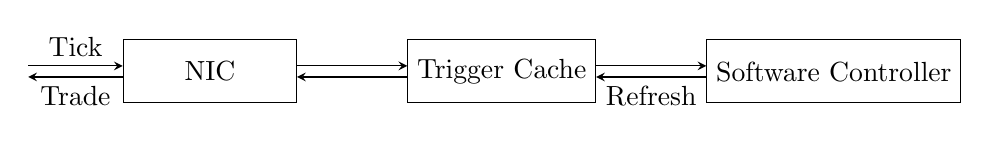
\begin{tikzpicture}[
	    box/.style={
		draw,
		minimum width=2.2cm,
		minimum height=0.8cm
	    },
	    >=stealth
	]
		\node[box] (nic) {NIC};
		\node[box, right=1.4cm of nic] (cache) {Trigger Cache};
		\node[box, right=1.4cm of cache] (controller) {Software Controller};

		% Tick / Trade
		\coordinate (tick) at ([xshift=-1.2cm,yshift=2pt]nic.west);
		\coordinate (trade) at ([xshift=-1.2cm,yshift=-2pt]nic.west);

		\draw[->] (tick) -- ([yshift=2pt]nic.west)
		    node[midway,above]{Tick};

		\draw[->] ([yshift=-2pt]nic.west) -- (trade)
		    node[midway,below]{Trade};

		% NIC <-> Trigger Cache
		\draw[->] ([yshift=2pt]nic.east) -- ([yshift=2pt]cache.west);
		\draw[->] ([yshift=-2pt]cache.west) -- ([yshift=-2pt]nic.east);

		% Trigger Cache <-> Software Controller
		\draw[->] ([yshift=2pt]cache.east) -- ([yshift=2pt]controller.west);
		\draw[->] ([yshift=-2pt]controller.west) -- ([yshift=-2pt]cache.east)
		    node[midway,below]{Refresh};
	\end{tikzpicture}
	\vspace{0.05cm}

	An onboard \textbf{trigger cache} lets us store parameters to determine how to respond to market data.

	Precomputing these before the latency-critical moment reduces hotpath latency.

	However, because of the large volume of market data and limited space in the trigger cache, \textbf{tick-to-config} latency/throughput are still important considerations. %Especially when you consider that market activity is autocorrelated
\end{frame}

%The cases when wire-to-wire matters (low jitter) are cases where marginal gains (but not necessarily step changes) are going to be not that useful. Can draw curves of opportunity vs latency.

\sectiondiagram{hardware}
\sectionquote{``All great events hang by a hair.'' Napoleon}
\section{Hardware Design}

\begin{frame}{Field Programmable Gate Arrays}
	%Xilinx introduced the first FPGA in 1985. Xilinx was acquired by AMD in 2022.
	\begin{center}
		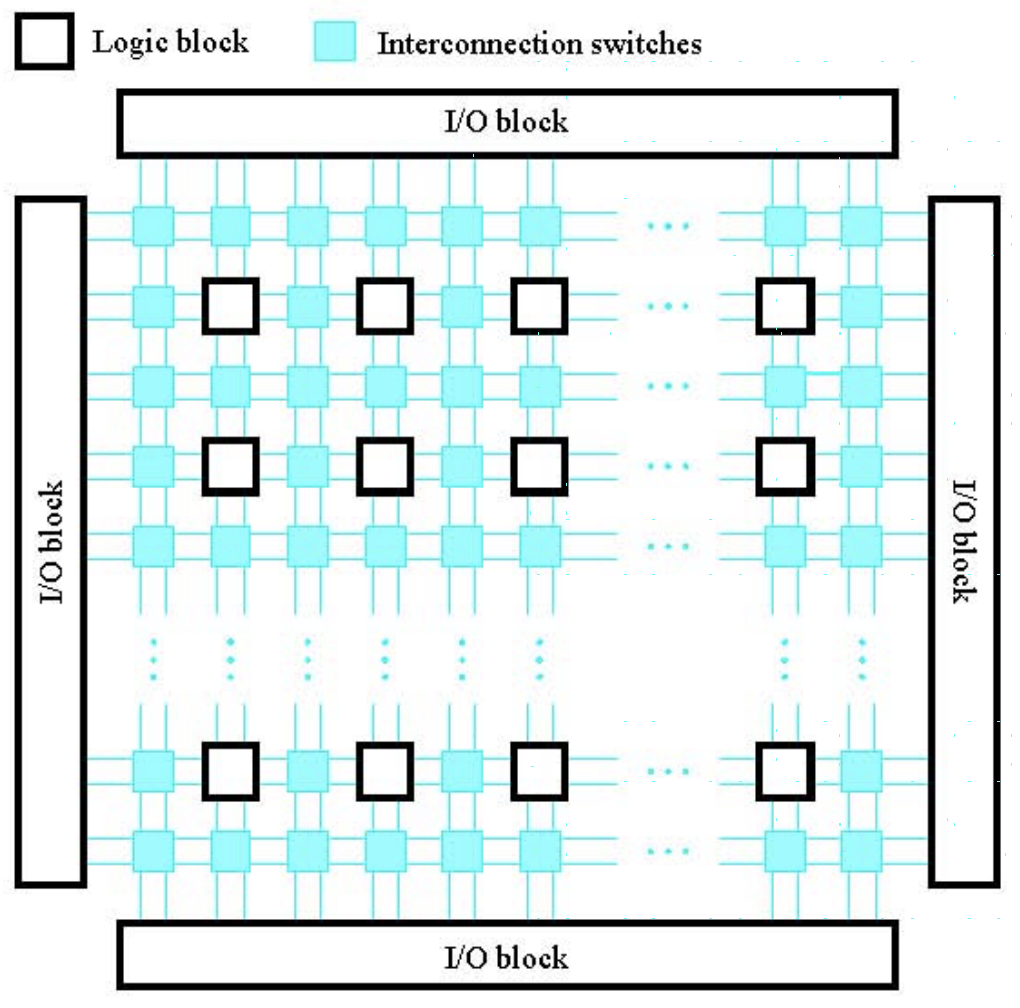
\includegraphics[scale=0.3]{assets/fpga.png}
	\end{center}
	While primarily useful onboard a NIC, FPGAs also have applications in other low-latency/high-throughput situations.
\end{frame}

\begin{frame}{Controllable Logic Blocks}
	\begin{center}
		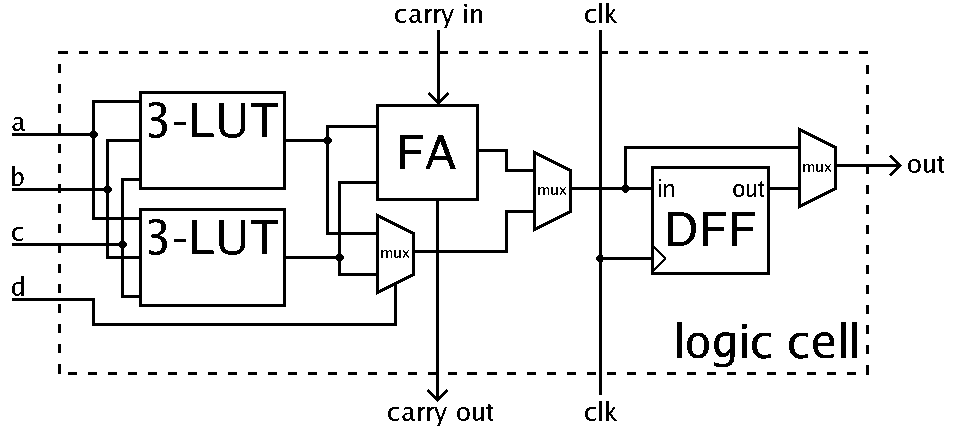
\includegraphics[scale=0.35]{assets/clb.png}
	\end{center}

	Different FPGAs will have different resources available in the CLB.

	For instance, the \href{https://docs.amd.com/r/en-US/Alveo-X3522PV-Adaptable-Accelerator-Card-User-Guide-UG1607/}{AMD Alveo X3522 NIC} uses \href{https://docs.amd.com/r/en-US/ug574-ultrascale-clb/CLB-Resources}{UG574 UltraScale+ CLBs}.
\end{frame}

\begin{frame}[fragile]{Synchronous Design}
	Synchronous design involves updating \textbf{registers} according to \textbf{combinational functions} on each \textbf{clock edge}.

	\newsavebox\lstA
	\begin{lrbox}{\lstA}
\begin{lstlisting}[ basicstyle=\ttfamily\bfseries\scriptsize ]
module itch_volume #(
    parameter int NUM_STOCKS = 4
) (
    input logic clk, input logic valid,
    input logic [5:0] pos, input logic [7:0] data_byte,

    input logic [31:0] buy_threshold  [NUM_STOCKS],
    input logic [31:0] sell_threshold [NUM_STOCKS],

    output logic [31:0] buy_volume  [NUM_STOCKS],
    output logic [31:0] sell_volume [NUM_STOCKS],

    output logic buy_trigger,
    output logic sell_trigger,
    output logic [15:0] trigger_locate
);
\end{lstlisting}
	\end{lrbox}
	\href{https://edaplayground.com/x/9qhM}{\usebox{\lstA}}%Packet slicing, only read part of packet. Concept of a HDL

	The length of each \textbf{clock cycle} must be chosen so that data has time to propagate to the destination register. %Reduce complexity of each step

	\textbf{Clock domain crossings} must be separated by a specialised interface to avoid data corruption. %restricted by line bandwidth in some ways
\end{frame}

\begin{frame}{Parallelism}
	\begin{itemize}
		\item A single clock cycle permits simultaneous dataflow through multiple CLBs at once.
		\item Module will be equal to the number of clock cycles to produce an output, divided by the clock frequency
	\end{itemize}

	One extreme example of parallelism afforded by special-purpose circuitry is a \href{https://docs.google.com/spreadsheets/d/1ndaz7_nyNNiciWW2bAGFsjldRJw72Wh_dNt0qzXUdKs/}{\textbf{systolic array}}.
\end{frame}

\begin{frame}{Memory Blocks}
%memory: flipflops, LUTs, bram/dram/sram, ultraram, registers, external dram; memory bandwidth, read/write ports count, pipeline depth
\end{frame}

\begin{frame}{Memory}
	%memory controller
	%ddio
%RAM. What are the physical interfaces a RAM card offers
%clock skew -> smaller is faster
\end{frame}

\begin{frame}{Synthesis}
	Following design and verification, programming the board involves the following stages:
	\begin{enumerate}
		\item Parsing of the \textbf{hardware description} (e.g. VHDL, Verilog, Clash, Hardcaml) into an abstract representation at the \textbf{logic-gate level}%minimal area is nice
		\item Identifying the dependency DAG of register values over time (\textbf{register-transfer level})
		\item Translation into resources made available by the board, and optimising the placement of logic/routing for timing, power, etc. %also crosstalk
		\item Generating a \textbf{gate-level netlist} to be serialised and `flashed' onto the board
	\end{enumerate}
	Optimisation generally makes use of some \textbf{cost model}. Depending on the software used, it may be non-deterministic.%intel quartus uses simulated annealing but vivado is in theory deterministic

	%question. is it common to run out of resources
\end{frame}

\begin{frame}{High-Level Synthesis}
%https://en.wikipedia.org/wiki/High-level_synthesis
\end{frame}

%Hardware is expensive to buy, expensive to program, expensive to maintain. 

\begin{frame}{Interconnects and PCIe (Peripheral Component Interconnect Express)}
	\textbf{PCIe} is the most common way for specialised components (NIC, CPU, RAM, GPU, etc.) in a computer to communicate.%also provides power

	\begin{center}
		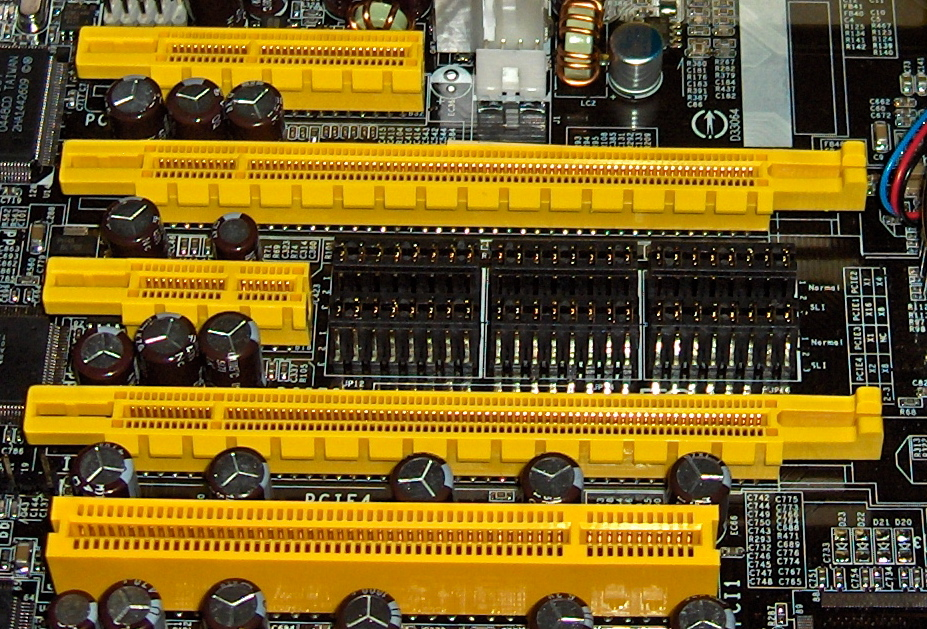
\includegraphics[scale=0.15]{assets/pcie.jpg}
	\end{center}

	\begin{itemize}
		\item OS/BIOS find components at startup and give them a \texttt{Bus:Device.Function} (BDF) address
		\item A clock signal is distributed from a central source for syncing
		\item Information is packetised, with the BDF address used for switching
		\item Packets carry \href{https://docs.amd.com/r/en-US/pg194-axi-bridge-pcie-gen3/PCIe-Transaction-Type}{transactions}, which can be reads, writes, interrupts etc.
	\end{itemize}
\end{frame}

\sectiondiagram{software}
\sectionquote{``You don't need to be an engineer to be a racing driver, but you do need Mechanical Sympathy.'' Jackie Stewart}
\section{Software Design}
\begin{frame}{Von Neumann Architecture}
	\begin{block}{}
		``In analyzing the functioning of the contemplated device, certain classificatory distinctions suggest themselves immediately. \ldots

		\begin{itemize}
			\item A \textbf{central arithmetical part} of the device will probably have to exist, and this constitutes the first specific part \ldots

			\item Second: The logical control of the device, that is the proper sequencing of its operations can be most efficiently carried out by a \textbf{central control organ} \ldots

			\item Third: Any device which is to carry out long and complicated sequences of operations (specifically of calculations) must have a considerable \textbf{memory}.''
		\end{itemize}

		John Von Neumann, 1945
	\end{block}
\end{frame}

\begin{frame}{CPUs}
	\begin{itemize}
		
	\end{itemize}


%fetch decode execute
%instruction pipelining, superscalar, `perf`
	%latency hiding https://news.ycombinator.com/item?id=26444397
%Overclocking https://www.blackcoretech.com/
\end{frame}

\begin{frame}{Microarchitecture}
%microarchitecture
%micro-ops. decoding is interpreting
%Tomasulo algo, reordering, out-of-order. eg store-and-load
%virtual registers
%google this, "cpu: prf rat rob rs bob mob"
%https://www.intel.com/content/www/us/en/docs/vtune-profiler/cookbook/2024-1/top-down-microarchitecture-analysis-method.html
\end{frame}

\begin{frame}{Caching}
%NUMA
%Swap memory as extreme case
%https://www.akkadia.org/drepper/cpumemory.pdf
%translation lookaside buffer; Cache invalidation, latency of different cache levels. LFU/LRU algorithm. Cache locality. https://www.youtube.com/watch?v=g_X5g3xw43Q
%"There are 2 hard problems in computer science: cache invalidation, naming things, and off-by-1 errors"
%Huge Pages https://www.hudsonrivertrading.com/hrtbeat/low-latency-optimization-part-1/
\end{frame}

\begin{frame}{Branch Prediction}
%Branch prediction incl perceptron-based. "Time forks perpetually toward innumerable futures." Borges
\end{frame}

\begin{frame}{Multi-Core Processing}
%cores, thread pinning, isolcpus, nohz_full
\end{frame}

\begin{frame}{Machine Instructions}
%Making fast machine code
%Profiling https://www.youtube.com/watch?v=EU_nQh8wg5A
%Profiler to identify unpredictable branches
%https://github.com/janestreet/magic-trace
%userspace timing
%simd
%https://github.com/david-grs/papipp
%cachegrind for counting cpu cycles https://stackoverflow.com/a/2588705
%flame graph
%x86 unique characteristics eg variable length
\end{frame}

\begin{frame}{Multitasking}
%OS-level stuff, three easy pieces, async programming
%userspace vs not
%The Path of A Packet Through the Linux Kernel https://www.net.in.tum.de/fileadmin/TUM/NET/NET-2024-04-1/NET-2024-04-1_16.pdf
%threaded code, pinned threads https://docs.kernel.org/admin-guide/kernel-per-CPU-kthreads.html
%atomics
%shared memory IPC
%https://access.redhat.com/documentation/en-us/red_hat_enterprise_linux_for_real_time/8/html-single/optimizing_rhel_8_for_real_time_for_low_latency_operation/index#proc_reducing-cpu-performance-spikes_optimizing-RHEL8-for-real-time-for-low-latency-operation
\end{frame}

\begin{frame}{Kernel Bypass}
%what even is a kernel
%interrupts (I think requires buffer to become full enough that NIC sends an interrupt) vs polling (constant checking)
%direct memory access
%TCPDirect, Onload, DPDK (+F-Stack or mTCP), VMA (vhost/Mellanox Messaging Accelerator), OpenOnload, RDMA/RoCE
\end{frame}

\begin{frame}{Algorithm Design}
%Time complexity picture. EMAs, exp weighted microprice (pose as a puzzle, whats best microprice update time complexity you can get with certain properties), etc.
\end{frame}

\begin{frame}{Memory Allocation}
	\centering
	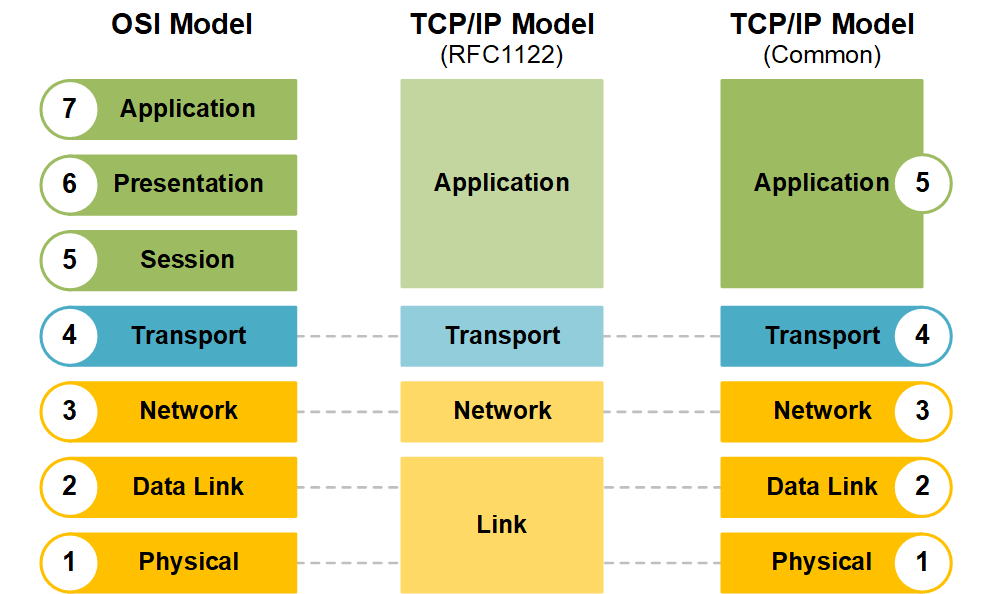
\includegraphics[scale=0.2]{assets/stack.png}
%static, automatic (stack), dynamic (heap)
%stack. fibonacci example. stack is still in RAM
%heap, garbage collection
%allocation in hotpath is expensive
% custom allocator https://www.youtube.com/watch?v=RpD-0oqGEzE
\end{frame}

% https://x.com/BrettHarrison/status/2084642796888015328?s=20
%structs, parsing
%interrupt storms
%Why linked lists suck
%x-free programming https://chatgpt.com/share/6a9817de-0990-83ec-b578-2bbf2ef877cb
%SIMD, multi-core systems. Parallelisation is nice
%
%https://docs.redhat.com/en/documentation/red_hat_enterprise_linux/6/html/performance_tuning_guide/main-network#s-network-future

\sectiondiagram{program}
\sectionquote{``There is no science apart from the general. \\ It may even be said that the very object of the exact sciences is to spare us these direct verifications.'' Henri Poincaré}
\section{Programming}
%### C++
% why compile instead of interpret. frontload work + checks to handle added complexity
%godbolt demo    https://www.youtube.com/watch?v=3W0vE_VKokY

%stack heap etc
%
%source
%efficient compilation eg makefiles
%AST
%compiler IR
%assembly
%instructions
%-O0 vs -O3
%inlining
%branch elimination & https://en.cppreference.com/cpp/language/attributes/likely
%virtual calls & devirtualisation using final keyword https://www.hudsonrivertrading.com/hrtbeat/optimising-compiler-performance-a-case-for-devirtualisation/
%bounds checks
%vectorisation
%profiler-guided optimisation
%
%optimising some actual code live. Start with how an exchange would implement a CLOB, and go to how a HFT would implement it.
%
%safety
% rust/ocaml/etc
%https://blog.janestreet.com/finding-memory-leaks-with-memtrace/
%

%start with the ethernet standard (and 10G docs), the TCP/UDP/IP RFCs, and lower level stuff like 64/66b and MAC/PHYs. Protocol docs like soupbinTCP, FIX/FIXP, ITCH/PITCH, MDP3, etc


\section{GPU Inference}
%## GPU inference
% https://x.com/BrettHarrison/status/1800954431552303225?s=20
%CUDA, warps
%talk about pros/cons of different GPU models, how to evaluate
%Why trees are slow. Universal approximation theorem does not apply for shallow forests.
%Fitting in memory. Quantisation, multiple GPUs (sharding), etc.; cross-sectional common components; state-based models for O(n) sequence processing. Caching model components with no new info.

%TPUs, systolic arrays

\section{Bibliography}
\begin{frame}{Useful}
	\begin{itemize}
		\item 
	\end{itemize}
\end{frame}

\begin{frame}{Classics \& Mentioned}
	\begin{itemize}
		\item 
	\end{itemize}
\end{frame}
\end{document}

%talk is free of AI slop
%
%
%Note existence of previous talk

%throughout, give some idea of the order of magnitude of latency we are dealing with

%"Eternity is in love with the productions of time." William Blake
%"Truth was the only daughter of Time." Leonardo da Vinci
%"Time drives everything before it, and is able to bring with it good as well as evil, and evil as well as good." Niccolò Machiavelli,
%"Time is the most valuable thing a man can spend." Theophrastus
%"Time is a necessary representation, lying at the foundation of all our intuitions ... In it alone is all reality of phænomena possible. These may all be annihilated in thought, but time itself, as the universal condition of their possibility, cannot be so annulled." Kant
%"Capital, in its ultimate self-definition, is nothing beside the abstract accelerative social factor. Its positive cybernetic schema exhausts it.  Runaway consumes its identity." Nick Land
%"Entropy and extropy have opposing time-signatures, so that time-reversal is a relatively banal cosmological fact. ‘We’ inhabit a bubble of backwards time (whoever we are), whilst immersed in a cosmic environment which runs overwhelmingly in the opposite direction. If reality is harsh and strange, that’s why." Nick Land
%"You cannot conquer Time." W. H. Auden
%"Nature to be commanded must be obeyed; and that which in contemplation is as the cause is in operation as the rule." Francis Bacon
%"I often say that when you can measure what you are speaking about, and express it in numbers, you know something about it; but when you cannot measure it, when you cannot express it in numbers, your knowledge is of a meagre and unsatisfactory kind; it may be the beginning of knowledge, but you have scarcely, in your thoughts, advanced to the stage of science, whatever the matter may be." William Thomson, Lord Kelvin
%"As eternity is reckoned, there's a lifetime in a second." Piet Hein
%"To every thing there is a season, and a time to every purpose under the heaven ... A time to get, and a time to lose; a time to keep, and a time to cast away." Ecclesiastes
%"Time is not composed of indivisible nows any more than any other magnitude is composed of indivisibles." Aristotle
%("Ease and speed in doing a thing do not give the work lasting solidity or exactness of beauty." Plutarch, Life of Pericles.)
%"Science is what we understand well enough to explain to a computer. Art is everything else we do." Donald Knuth
%\sectionquote{``When wireless is perfectly applied the whole earth will be converted into a huge brain, which in fact it is, all things being particles of a real and rhythmic whole.'' Nikola Tesla}
%\sectionquote{``Science is when it works but shouldn’t. Engineering is when it doesn’t work but should.'' Sam Altman}
%"being so many different sizes in a day is very confusing" alice in wonderland
%\sectionquote{``Time is the inexorable process of doing computation.'' Stephen Wolfram}



%https://databento.com/blog/introduction-matching-engines
%https://api2.sgx.com/sites/default/files/2026-06/OMnet_MessRef_SGX_va42.pdf
%https://www.eecis.udel.edu/~mills/database/papers/history.pdf
%https://www.realclearmarkets.com/articles/2018/02/14/a_clear_market_fairness_issue_requires_a_clear_collective_response_103150.html
%https://www.synopsys.com/glossary/what-is-synthesis.html
%https://web.archive.org/web/20070623082626/http://qss.stanford.edu/%7Egodfrey/vonNeumann/vnedvac.pdf

%Relativity: https://en.wikipedia.org/wiki/One-way_speed_of_light#Einstein_convention

%https://www.youtube.com/watch?v=BVVNtG5dgks
%https://www.youtube.com/watch?v=g_X5g3xw43Q
%https://www.youtube.com/watch?v=I_TtMk5z0O0

%
%# Trading as an engineering problem. Why do you care?
%You get to build things that do things.
